\documentclass[11pt, oneside]{report}
\linespread{1.5}
\usepackage{graphicx}
\usepackage{xcolor}
\usepackage{amsmath}
\usepackage[super,sort&compress,comma]{natbib}
\usepackage{fancyhdr}
\usepackage{booktabs}
\usepackage{hyperref}
\usepackage{scrextend}
\usepackage{subcaption}
\usepackage{mhchem}

\fancyhf{}% Clear header/footer
\fancyhead[C]{\leftmark}% Right header
\fancyfoot[L]{}% Left footer
\fancyfoot[R]{\thepage}% Right footer
\fancyfoot[C]{DRAFT}

\pagestyle{fancy}

\usepackage[format=plain,
            labelfont={bf},
            textfont=it]{caption}

\usepackage{geometry}
\geometry{a4paper,left=40mm,top=30mm, right = 30mm, bottom = 30mm} 
\begin{document}
	
\setcounter{tocdepth}{1} 

\begin{titlepage}
\begin{center}
\vspace*{1cm}
 
\LARGE
\textbf{Disordered solids as next-generation cathode materials}
       
\vspace{0.5cm}
\normalsize       
submitted by
       
      
\Large
\textbf{Matt Clarke}
 
\vspace{0.5cm}
\normalsize
as a confirmation report towards the degree of\\
Doctor of Philosophy
 
\vspace{0.5cm}
       
\LARGE
University of Bath\\
\normalsize
Department of Chemistry\\
       
\vspace{0.8cm}
\today
       
\vfill
\large
\textbf{COPYRIGHT}
\end{center}
Attention is drawn to the fact that copyright of this thesis rests with the author. A
copy of this thesis has been supplied on condition that anyone who consults it is
understood to recognise that its copyright rests with the author and that they must
not copy it or use material from it except as permitted by law or with the consent of
the author.
\\
\\
This thesis may be made available for consultation within the University Library and may be photocopied or lent to other libraries for the purposes of consultation.

\vspace{2cm}
\noindent Signature of Author: \dotfill
   
\end{titlepage}
\tableofcontents
\listoffigures
\chapter{Introduction}
\section{Background: energy storage}
The demand for ever improving energy storage solutions is driven by both commercial interests and an urgent societal need.
In order to curtail \ce{CO2} emissions and limit the impact of global warming, a shift from fossil-fuel based energy generation towards renewable energy is vital.\cite{Goodenough2013}
Unfortunately, a characteristic of many renewable energy sources, such as wind and solar energy, is the intermittent nature of its generation.\cite{Goodenough2010a,Ellis2012,Liu2013}
As such, it is necessary to decouple the generation and consumption of the energy produced by these means via intermediate storage.

Vehicle electrification may displace conventional combustion engine driven transport, another major source of greenhouse gases and pollution.\cite{Blomgren2017}
While some commercial success has being enjoyed for electric vehicles in recent years, concerns surrounding safety, longevity, and insufficient energy density to overcome the ``range anxiety'' of most consumers demands further development of battery technologies for widespread adoption of electric vehicles to occur.\cite{Cano2018a,Schmuch2018}

Finally, consumer demand for increasingly powerful, thin, and light portable electronics with larger times between charges has pushed current battery chemistries to their limits.\cite{Liu2010}
With the majority of developments in batteries for portable electronics in recent years arising not from improvements in their chemistries, but by improved manufacturing processes with diminishing returns, the need for a fundamentally different battery chemistry may arise in the near future.
Indeed, in recent years a number of manufacturers have, in a drive to yield more performance from the same fundamental chemistries, produced cells which ultimately proved to be unsafe.\cite{Loveridge2018}

Any given use case will prioritise different properties in their energy storage solutions, requiring fundamentally different battery chemistries to be developed and improved upon.

\section{Li-ion batteries}
\renewcommand{\thefootnote}{\fnsymbol{footnote}}
Lithium, being the lightest and most electropositive metal,\cite{Tarascon2010} is well suited to applications in high density energy storage.
The first commercial Li-ion battery was developed in the 1980's by John Goodenough\cite{Mizushima1981} and manufactured by Sony Co. in 1991.\cite{Li2018}
This development, coupled with the rapid decrease in the size of transistors, sparked the portable electronics revolution.
In the years since, a range of battery chemistries have been developed, tailored to specific applications.

\subsection{Anatomy of an electrochemical cell}
Figure \ref{fig:Goodenough} illustrates a typical electrochemical cell, specifically the first commercial Li-ion battery.
The cell consists of an anode and cathode\footnote{It is conventional when discussing battery materials to refer to the electrode which is positive during discharge as the anode, and that which is negative as the cathode.},
which are electrically isolated from one another, but able to freely exchange ions via an electrolyte.
The cell is charged by applying an external potential across the cell, forcing electrons to the anode.
\ce{Li+} ions are extracted from the \ce{LiCoO2} cathode, diffuse between the electrodes via an electrolyte (\ce{LiFP6 in organic solvent} typically), and intercalate into the anode structure to maintain charge neutrality.

During discharge, the reverse process occurs.
\ce{Li+} ions driven by a difference in chemical potential move from the anode to the cathode, and electrons travel via an external circuit to maintain charge neutrality, allowing useful work to be done.


\begin{figure}
\centering
\begin{subfigure}{\linewidth}
  \centering
  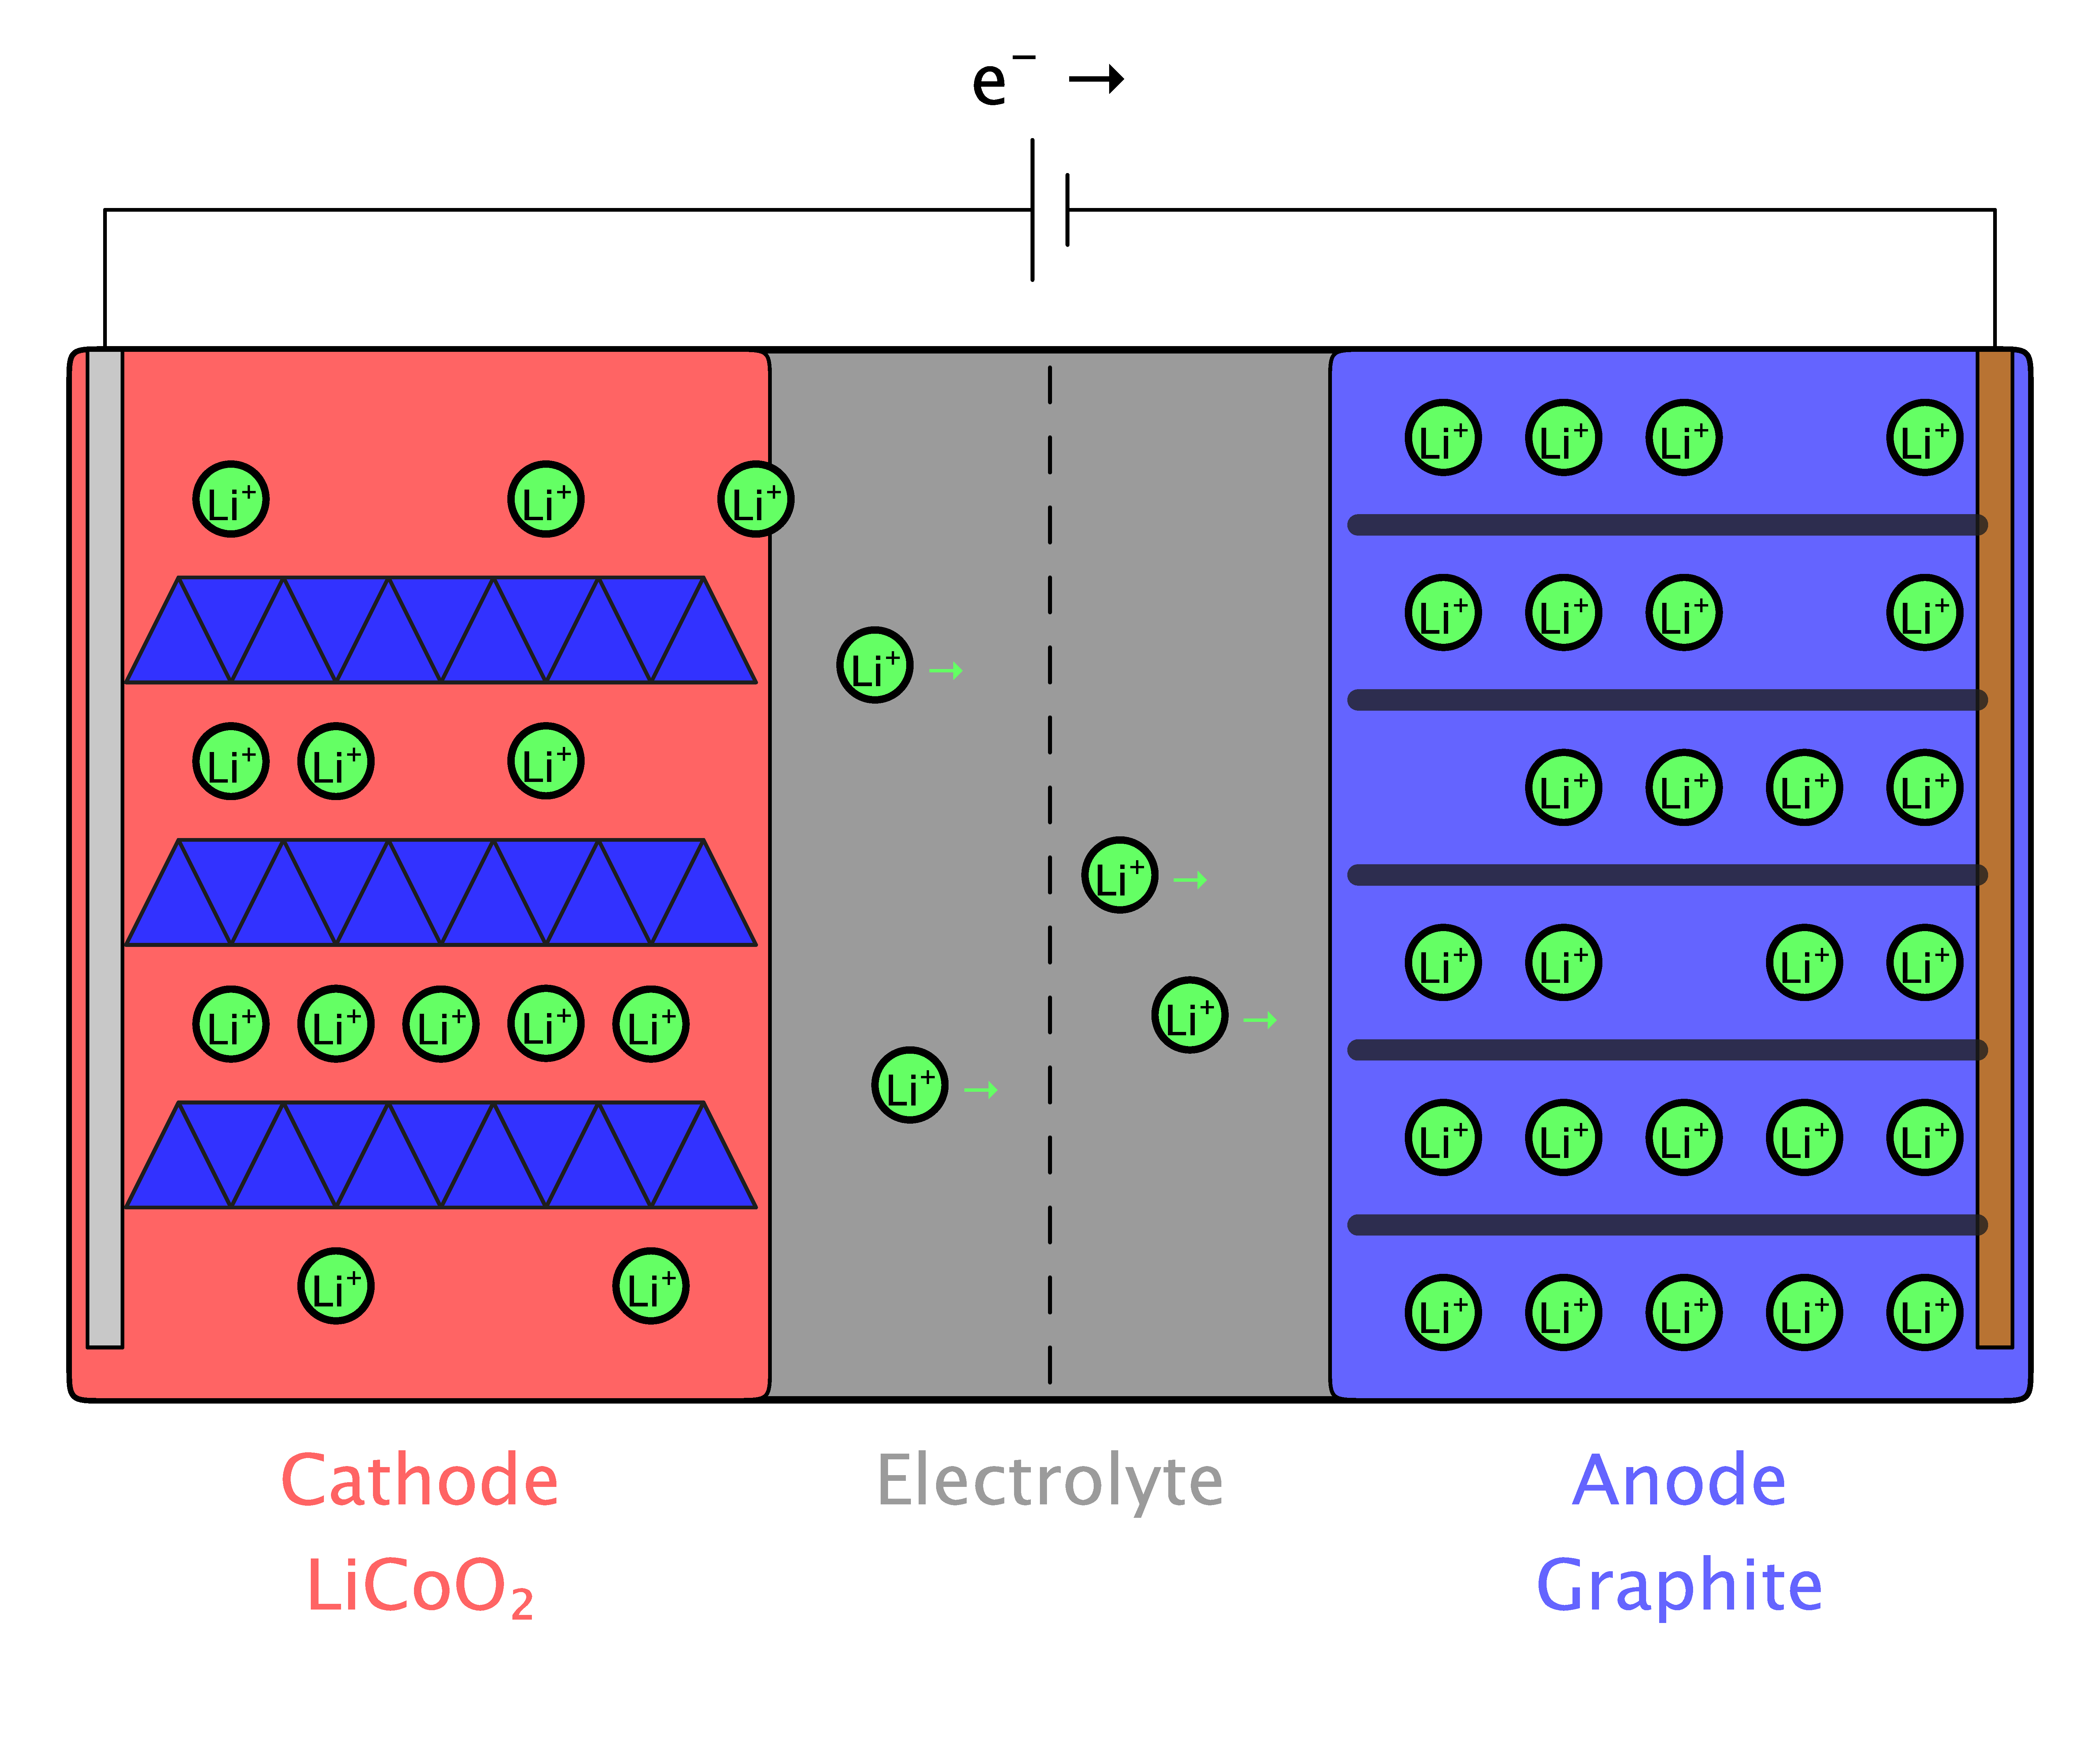
\includegraphics[width=0.7\linewidth, trim=1cm 1cm 1cm 1cm, clip]{figures/batteryCharge/batteryCharge}
  \caption{Charging}
  \label{fig:GoodenoughCharging}
\end{subfigure}

\begin{subfigure}{\linewidth}
  \centering
  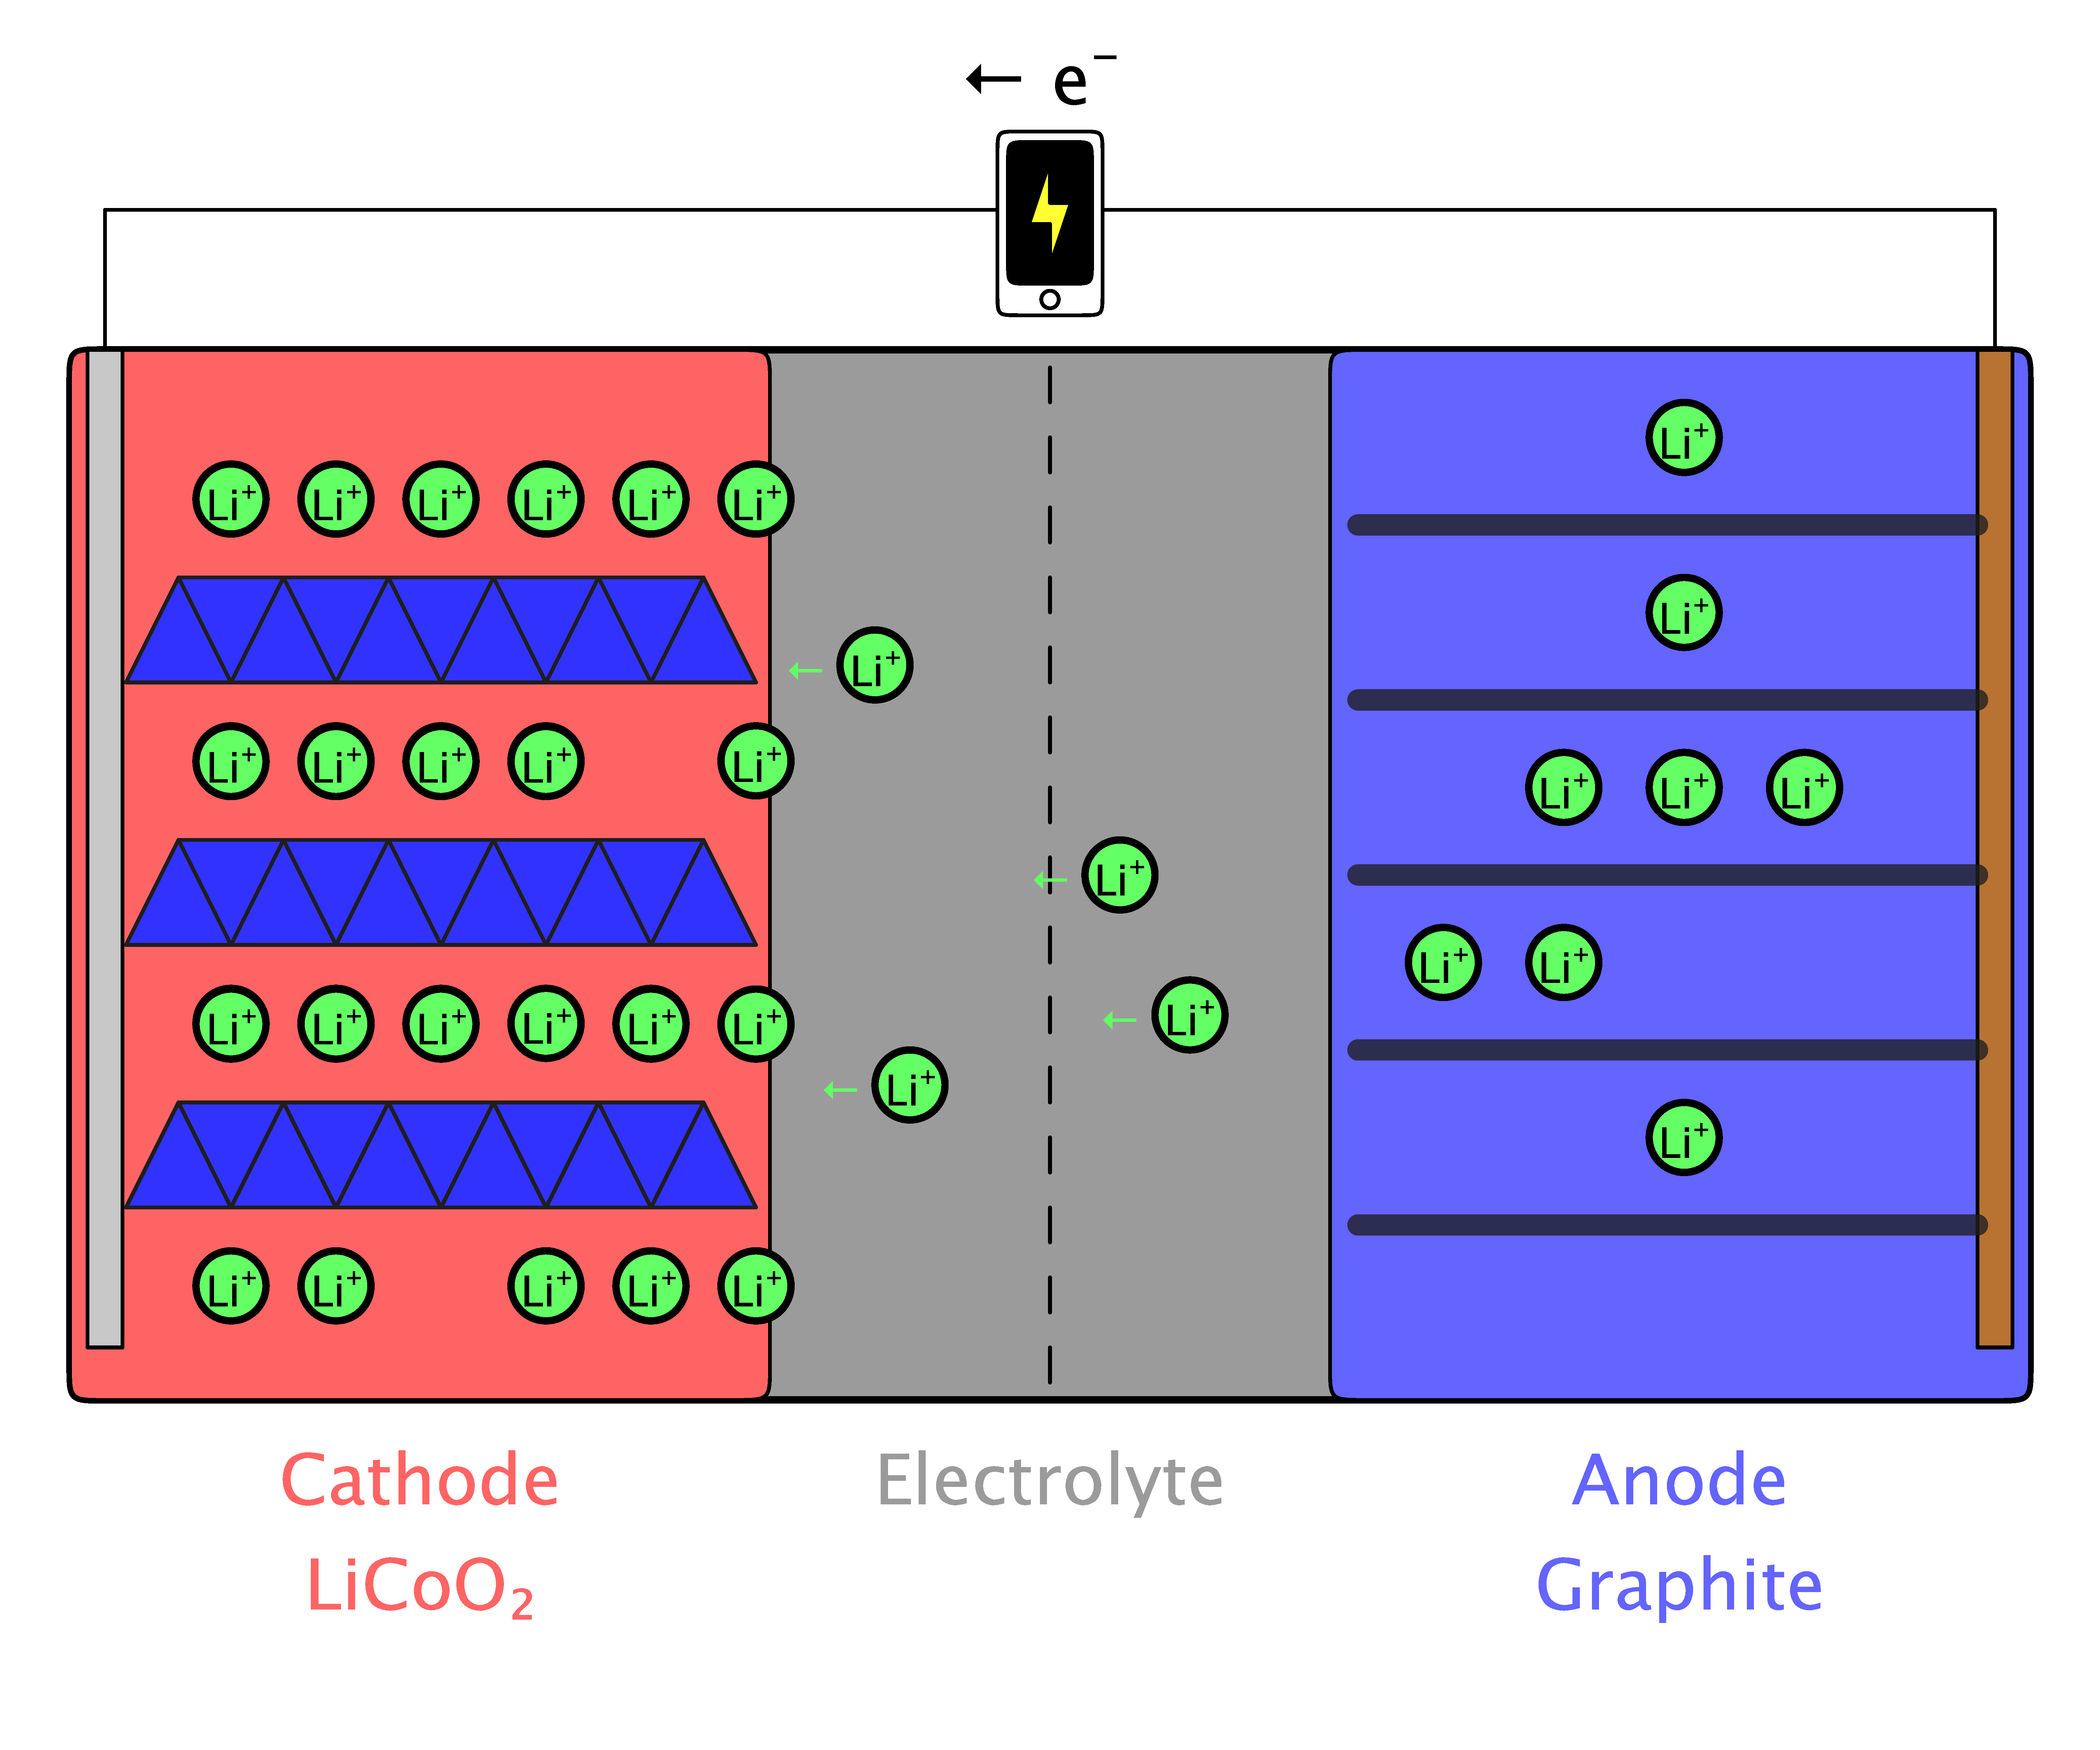
\includegraphics[width=0.7\linewidth, trim=1cm 1cm 1cm 1cm, clip]{figures/batteryDischarge/batteryDischarge}
  \caption{Discharging}
  \label{fig:GoodenoughDischarging}
\end{subfigure}
\caption[Li-ion battery schematic]{A schematic of a common Li-ion battery. During charging (a), electrons are driven to the anode by an external potential. \ce{Li+} ions move from the cathode to the anode to maintain charge neutrality. During discharge (b), \ce{Li+} ions are driven to the cathode by a difference in chemical potential. As the electrodes are electrically isolated from one another by the separator, electrons are instead forced to travel via an external circuit and provide work.} 
\label{fig:Goodenough}
\end{figure}

\newpage
\section{Electrolyte materials}
In order for useful work to be yielded from batteries, and in order to prevent short circuiting, the electrodes must be electrically isolated from one another.\cite{Palacin2009}
In practice, this is implemented by use of a porous but electrically insulating separator material (typically a multilayer polymer) coupled with an electrolyte material.
As the rate at which the battery can discharge is dependant on the rate at which the electrodes can exchange \ce{Li+} ions, high ionic conductivity is vital for commercially viable electrolytes.


\subsection{Liquid electrolytes}
All Li-ion battery systems currently available commercially use liquid electrolytes.\cite{Famprikis2019}
These typically consist of \ce{LiFP6} salts dissolved in a mixture of organic solvents.
The exact composition will vary dependant on the choice of electrodes, application, and manufacturer.
That said, the use of ethyl methyl carbonate (EC) is universal in organic electrolytes, as its inclusion results in the formation of a passivating layer on graphite anodes, preventing solvent molecules from intercalating into the anode and destroying the graphitic structure.\cite{Palacin2009}

These electrolyte solutions are typically stable to \SI{3.5}{\volt}, above which the electrolyte decomposes in a kinetically limited process.
As conventional batteries are often charged above \SI{3.5}{\volt}, this causes a slow decline in the performance of the battery over time.
The use of hierarchical electrode materials may mitigate this issue and allow the use of higher voltage cathode chemistries. \cite{Zhou2018}

\subsection{Solid electrolytes}
Solid-state batteries have been of significant research interest in recent years, primarily due to the increased safety they can offer.\cite{Famprikis2019, Zhang2018, Manthiram2017a, Janek2016}
Liquid electrolytes typically consist of highly flammable organic solvents which lead to dangerous failure modes.
The use of such electrolytes in EV applications, where mechanical failure of batteries is likely in the event of a crash, can significantly enhance the safety of EV's.

They can also offer higher energy densities, by enabling the use of higher energy density electrode materials which cannot be in liquid electrolyte systems.
In particular, they may allow the use of Li-metal anodes (see Section \ref{sec:anodes}), increasing the energy density of the anode by an order of magnitude,\cite{Zhang2018} and high voltage cathode materials for which no known stable liquid electrolyte exists.

\section{Anode materials}
\label{sec:anodes}
Li metal is theoretically the best possible anode material with a huge theoretical capacity (\SI{3860}{\milli\ampere\hour\per\gram}/\SI{2061}{\milli\ampere\hour\per\centi\meter\cubed}), and was used in early Li battery research. 
Unfortunately, dendrite formation at the anode surface ultimately leads to short circuiting and fires, preventing its use with current commercially viable electrolytes. \cite{Cheng2017,Guo2017a,Lin2017,Placke2017}
As such, current commercial batteries generally use a graphitic anode which undergoes the following reversible reaction:\cite{Islam2014}
\begin{equation}
\ce{Li_xC6(s) <-> $x$Li+(soln) +6C(s) + $x$e-}
\end{equation}
The performance of graphite anodes is a function of their morphology,\cite{Buqa2005} meaning the capacity achieved is strongly influenced by the manufacturing processes used and the state of health of the battery.

The use of graphite (albeit value-added graphite) as a key material in batteries is of course a huge advantage due to its high abundance, low cost, and excellent electrical conductivity.
Whilst the graphite anodes are not the current limiting factor in commercial batteries, having higher capacities (\SI{372}{\milli\ampere\hour\per\gram}) than the best available cathodes, they are still of research interest in anticipation of next-generation cathodes.

Tin and silicon based alloys offer higher capacities than graphite, but are currently not viable due to myriad issues including large volume changes (+200\% for Si) over a charge/discharge cycle.\cite{Scrosati2011}

\newpage
\section{Cathode materials}
Cathode materials are currently the limiting factor in commercial batteries, making them a highly active and rapidly changing field of research.\cite{Marom2011}
While a wide range of materials are currently of research interest, only a few classes of cathode materials have enjoyed widespread commercialisation thus far.

\subsection{\ce{LiMO2}}
\begin{figure}
\centering
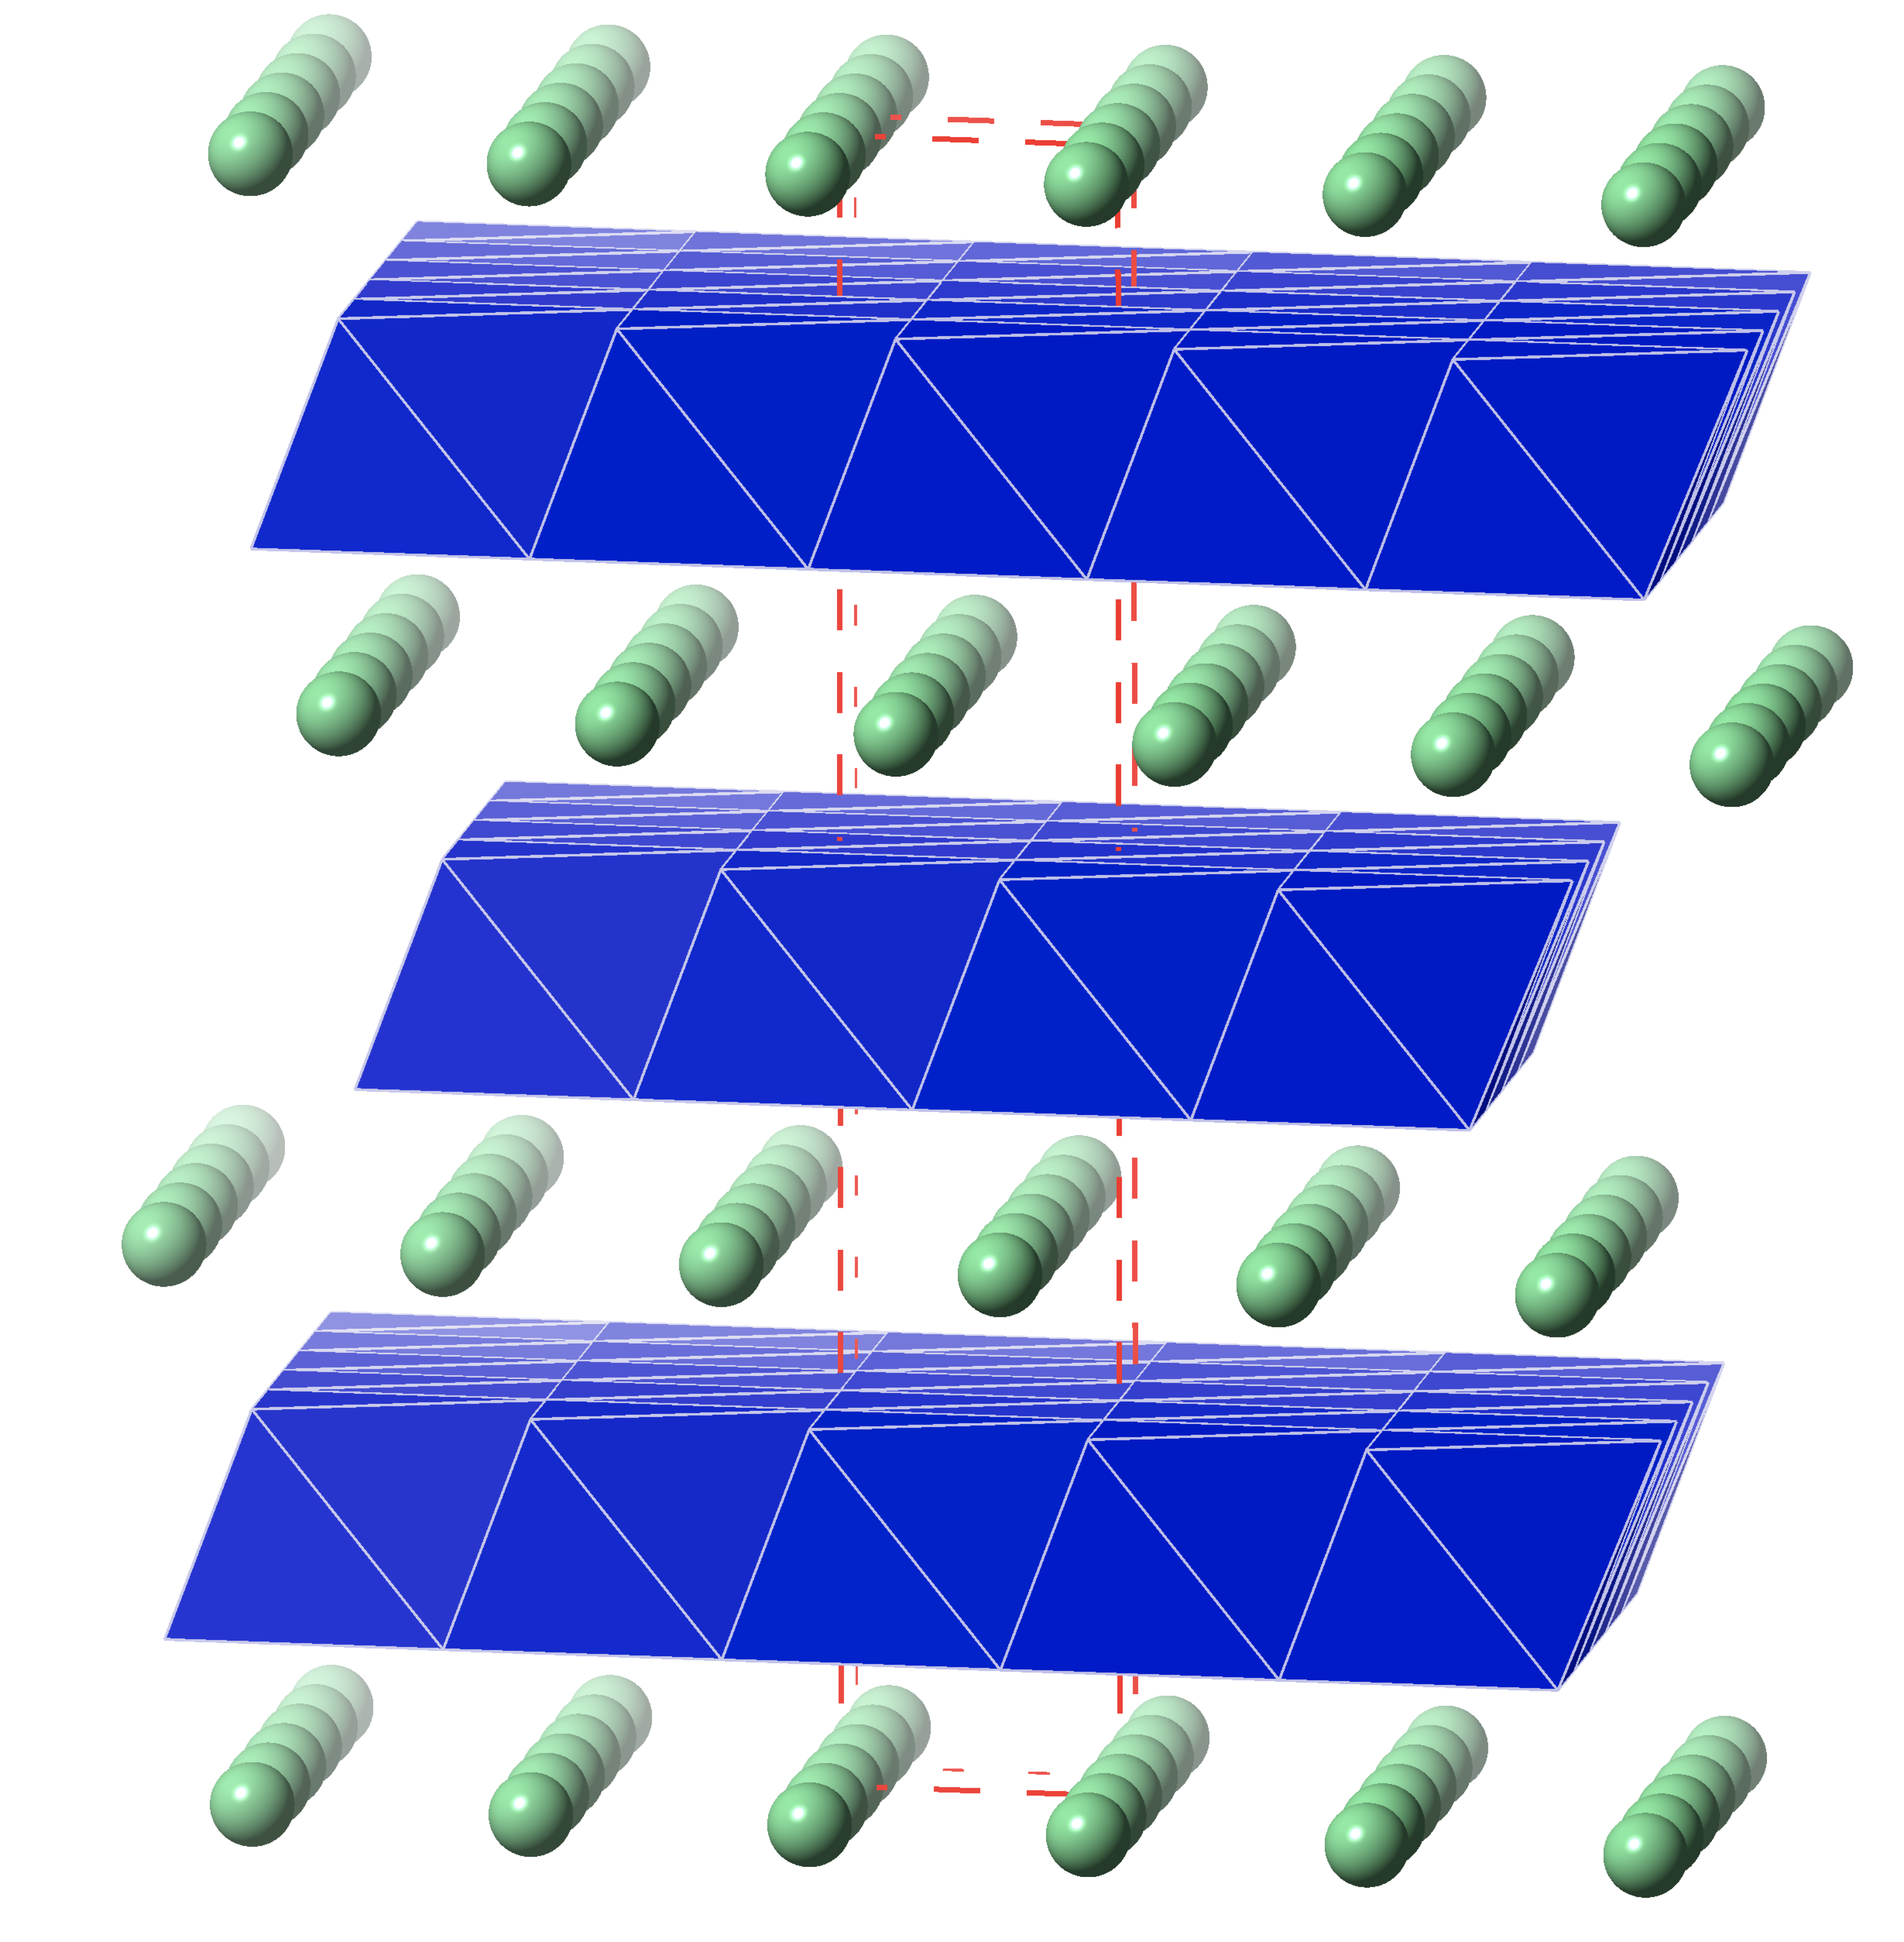
\includegraphics[height=0.6\linewidth]{figures/structures/LiCoO2}
\caption[Layered \ce{LiMO2} structure]{Layered \ce{LiMO2} structure. (\ce{Li+} ions: green; \ce{MO6} octohedra: blue)\\ }
\label{fig:LCO}
\end{figure}
\ce{LiMO2} adopt \ce{\alpha-NaFeO2} structures (Figure \ref{fig:LCO}), which is the prototype structure of \ce{AMO2} layered cathode materials.
The structure is comprised of alternating layers of \ce{[CoO2]-} and \ce{Li+} layers ($R\bar{3}M$).\cite{Islam2014}
The low migration barrier between adjacent \ce{Li+} sites within each layer leads to fast 2D ion transport through the structure.\cite{Ellis2010a}
The reaction occurring as lithium is reversibly extracted from \ce{LiMO2} cathodes can be written as:\cite{Islam2014}
\begin{equation}
\ce{Li_{1-x}MO2(s) +$x$Li+(soln) +$x$e- <=> LiMO2(s)}
\end{equation}

Different metals allow for a larger fraction of Li to be reversibly extracted, corresponding to higher energy densities.

\paragraph{\ce{LiCoO2}}
As shown in Figure \ref{fig:Goodenough}, the first commercial rechargeable Li-ion battery used a \ce{LiCoO2} (LCO) cathode (Figure \ref{fig:LCO}).
Its capacity of around \SI{150}{\milli\ampere\hour\per\gram} constituted a step change from its predecessors when it was introduced in the 1990's, and it remains prevalent in commercial applications today, particularly in portable electronics.\cite{Goodenough2013}

That said, a number of issues exist with LCO cathodes.
Firstly, the delithiation of the cathode is only reversible up to 50 \% removal of the total Li, thus around half of the theoretical capacity (\SI{275}{\milli\ampere\hour\per\gram}) cannot be reversibly accessed.\cite{Rozier2015}
Additionally, there are a number of ethical, economic, and sustainability issues associated with the supply of cobalt,\cite{Mauger2017, Larcher2015} driving research into layered metal oxide chemistries using other metals:\cite{Rozier2015}

\begin{labeling}{\textbf{\ce{LiMnO2}}}
	\item [\textbf{\ce{LiNiO2}}] Despite being cheaper, more sustainable, and having a higher theoretical capacity (\SI{200}{\milli\ampere\hour\per\gram}) than \ce{LiCoO2}, the low thermal stability of lithium nickel oxide cathodes in the presence of organic electrolytes poses a significant safety risk, making it unsuitable for commercial applications.
	Furthermore, it is not easily synthesised due to the formation of non-stoichiometric compounds arising from the spontaneous reduction of \ce{Ni^3+} to  \ce{Ni^2+}, resulting in \ce{Ni^2+} ions on \ce{Li+} sites.\cite{Das2017}
	\item [\textbf{\ce{LiMnO2}}] The similarity of the ionic radii of high-spin \ce{Mn^3+} (\SI{0.65}{\angstrom}) and \ce{Li+} (\SI{0.76}{\angstrom}) prevents the formation of stable layered \ce{LiMnO2}.\cite{Rozier2015,Rossen1992}
	While metastable \ce{LiMnO2} can be synthesised, the more stable \ce{LiMn2O4} forms upon cycling, giving poor electrochemical performance.
\end{labeling}

\newpage
\subsection{Mixed-metal layered \ce{LiMO2}}
A strategy to incorporate some of the benefits of \ce{LiNiO2}, whilst overcoming the stability and synthesis issues which have prevented its practical use is the partial substitution of Ni for other metals.\cite{Rozier2015}
Binary and ternary \ce{LiMO2} have been extensively studied, yielding compounds which have enjoyed commercial success.
Each of the below compounds have the same layered structure as \ce{LiCoO2} shown in Figure \ref{fig:LCO}, with the occupancy of each metal site determined by the stoichiometry of the mixed-compounds, and any relevant cation ordering effects.

\paragraph{\ce{Li[Ni_{1-y-z}Co_yAl_z]O2} (NCA)}
The issues with \ce{LiNiO2} arise due to the instability of \ce{Ni^3+} at elevated temperatures, and the similar ionic radii of \ce{Ni^2+} and \ce{Li+} causing migration of \ce{Ni} into the \ce{Li} layers.\cite{Das2017}
\ce{Li[Ni_{1-y-z}Co_yAl_z]O2} (NCA) type cathodes overcome these issues through the partial substitution of \ce{Ni^3+} with \ce{Co^3+} and \ce{Al^3+}:
\begin{labeling}{\textbf{\ce{Co^3+}}}
\item [\textbf{\ce{Co^3+}}] The addition of \ce{Co^3+} stabilises \ce{Ni^3+} at elevated temperatures, minimising the formation of \ce{Ni^2+}.
The similar ionic radii of \ce{Co^3+} (\SI{0.545}{\angstrom}) and \ce{Ni^3+} (\SI{0.56}{\angstrom}) allows the formation of \ce{Li(Ni,Co)O2} solid solutions.\cite{Rozier2015}
The large difference in ionic radii of these species with \ce{Li+} leads to M/Li ordering and stable layered oxides.

\item [\textbf{\ce{Al^3+}}] \ce{Al^3+} cations occupy M sites in the \ce{MO2} layers.
The stronger \ce{Al-O} bonds (relative to \ce{Co-O} and \ce{Ni-O}) serve to stabilise the cathode structure, enhancing its cycling performance and stability at high voltages.
This also enhances thermal stability, overcoming a significant barrier to the use of \ce{LiNiO2}.
As \ce{Al} is electrochemically inert, its inclusion is detrimental to the overall capacity of the cathode.
\end{labeling}

The drawbacks of including expensive Co, and inert Al are outweighed by the benefits offered by a viable layered nickel oxide cathode.
As such, \ce{LiNi_{0.8}Co_{0.15}Al_{0.05}O2} has enjoyed wide commercial success in EV applications (Tesla) with a high discharge capacity (\SI{200}{\milli\ampere\hour\per\gram}) compared to LCO.
\cite{Nitta2015}



\newpage

\begin{figure}
\centering
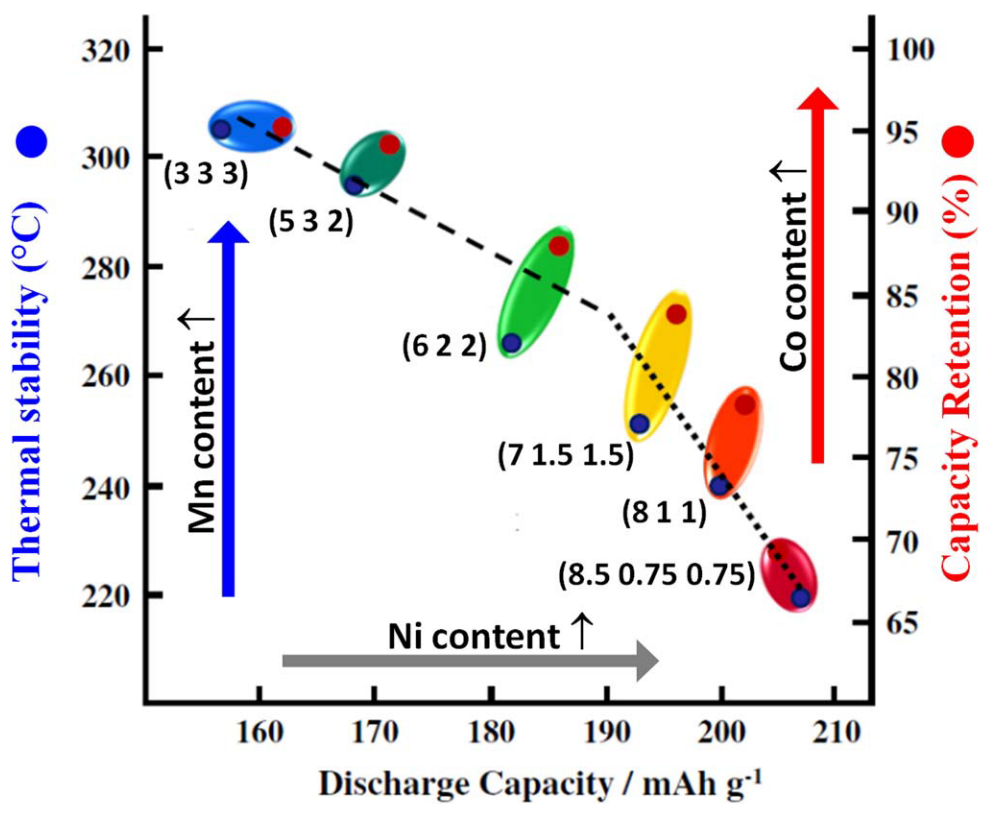
\includegraphics[width=0.5\linewidth]{figures/static/NMC_composition}

\caption[Key properties of NMC as a function of metals ratio]{Key properties of NMC as a function of metals ratio.\cite{Rozier2015, Noh2013}} 
\label{fig:NMCcomp}
\end{figure}

\paragraph{\ce{Li[Ni_{1-y-z}Mn_yCo_z]O2} (NMC)}
Initially overlooked as a poor cathode candidate when it was first reported in 1992,\cite{Rossen1992} \ce{Li[Ni_{1-x}Mn_x]O2} cathodes were revisited and expanded on in the early 2000's.\cite{Lu2001,Yabuuchi2008, Venkatraman2004}.
Whilst high temperature synthesis overcame issues associated with cation distribution,\cite{Hinuma2007} the tendency for the Ni and Mn to be in 2+ and 4+ oxidation states respectively gave rise to the same issues seen in \ce{LiNiO2}, namely \ce{Ni^2+} in the Li layer.
This meant that the high capacities observed \SI{200}{\milli\ampere\hour\per\gram} in \ce{Li[Ni_{0.5}Mn_{0.5}]O2} were only accessible at low discharge rates due to inhibited Li migration, limiting the practicality of this material as a cathode.

As with LCA, the partial substitution of \ce{Ni} for \ce{Co} limited the formation of \ce{Ni^2+} in the Li layer, leading to the \ce{Li[Ni_{1-y-z}Mn_yCo_z]O2} (NMC) class of materials.
\ce{Li[Ni_{1/3}Mn_{1/3}Co_{1/3}]O2} (NMC-111, named for the Ni:Mn:Co ratio) is currently commercialised with a practical reversible capacity of \SI{180}{\milli\ampere\hour\per\gram}.

Figure \ref{fig:NMCcomp} shows the discharge capacity, thermal stability, and capacity retention for various NMC compositions.
Broadly speaking, the discharge capacity of the material is improved by increased Ni content, the thermal stability improved by increased Mn content, and the capacity retention improves with increasing Co content.
As such, research efforts focusing on retaining high capacity retention and thermal stabilities at higher Ni concentrations are plentiful.
One promising strategy to achieve this is the formation of hierarchical cathode particles, with high capacity Ni-rich cores and stable Mn-rich shells. \cite{Zhou2018}
\newpage
\begin{figure}
\centering
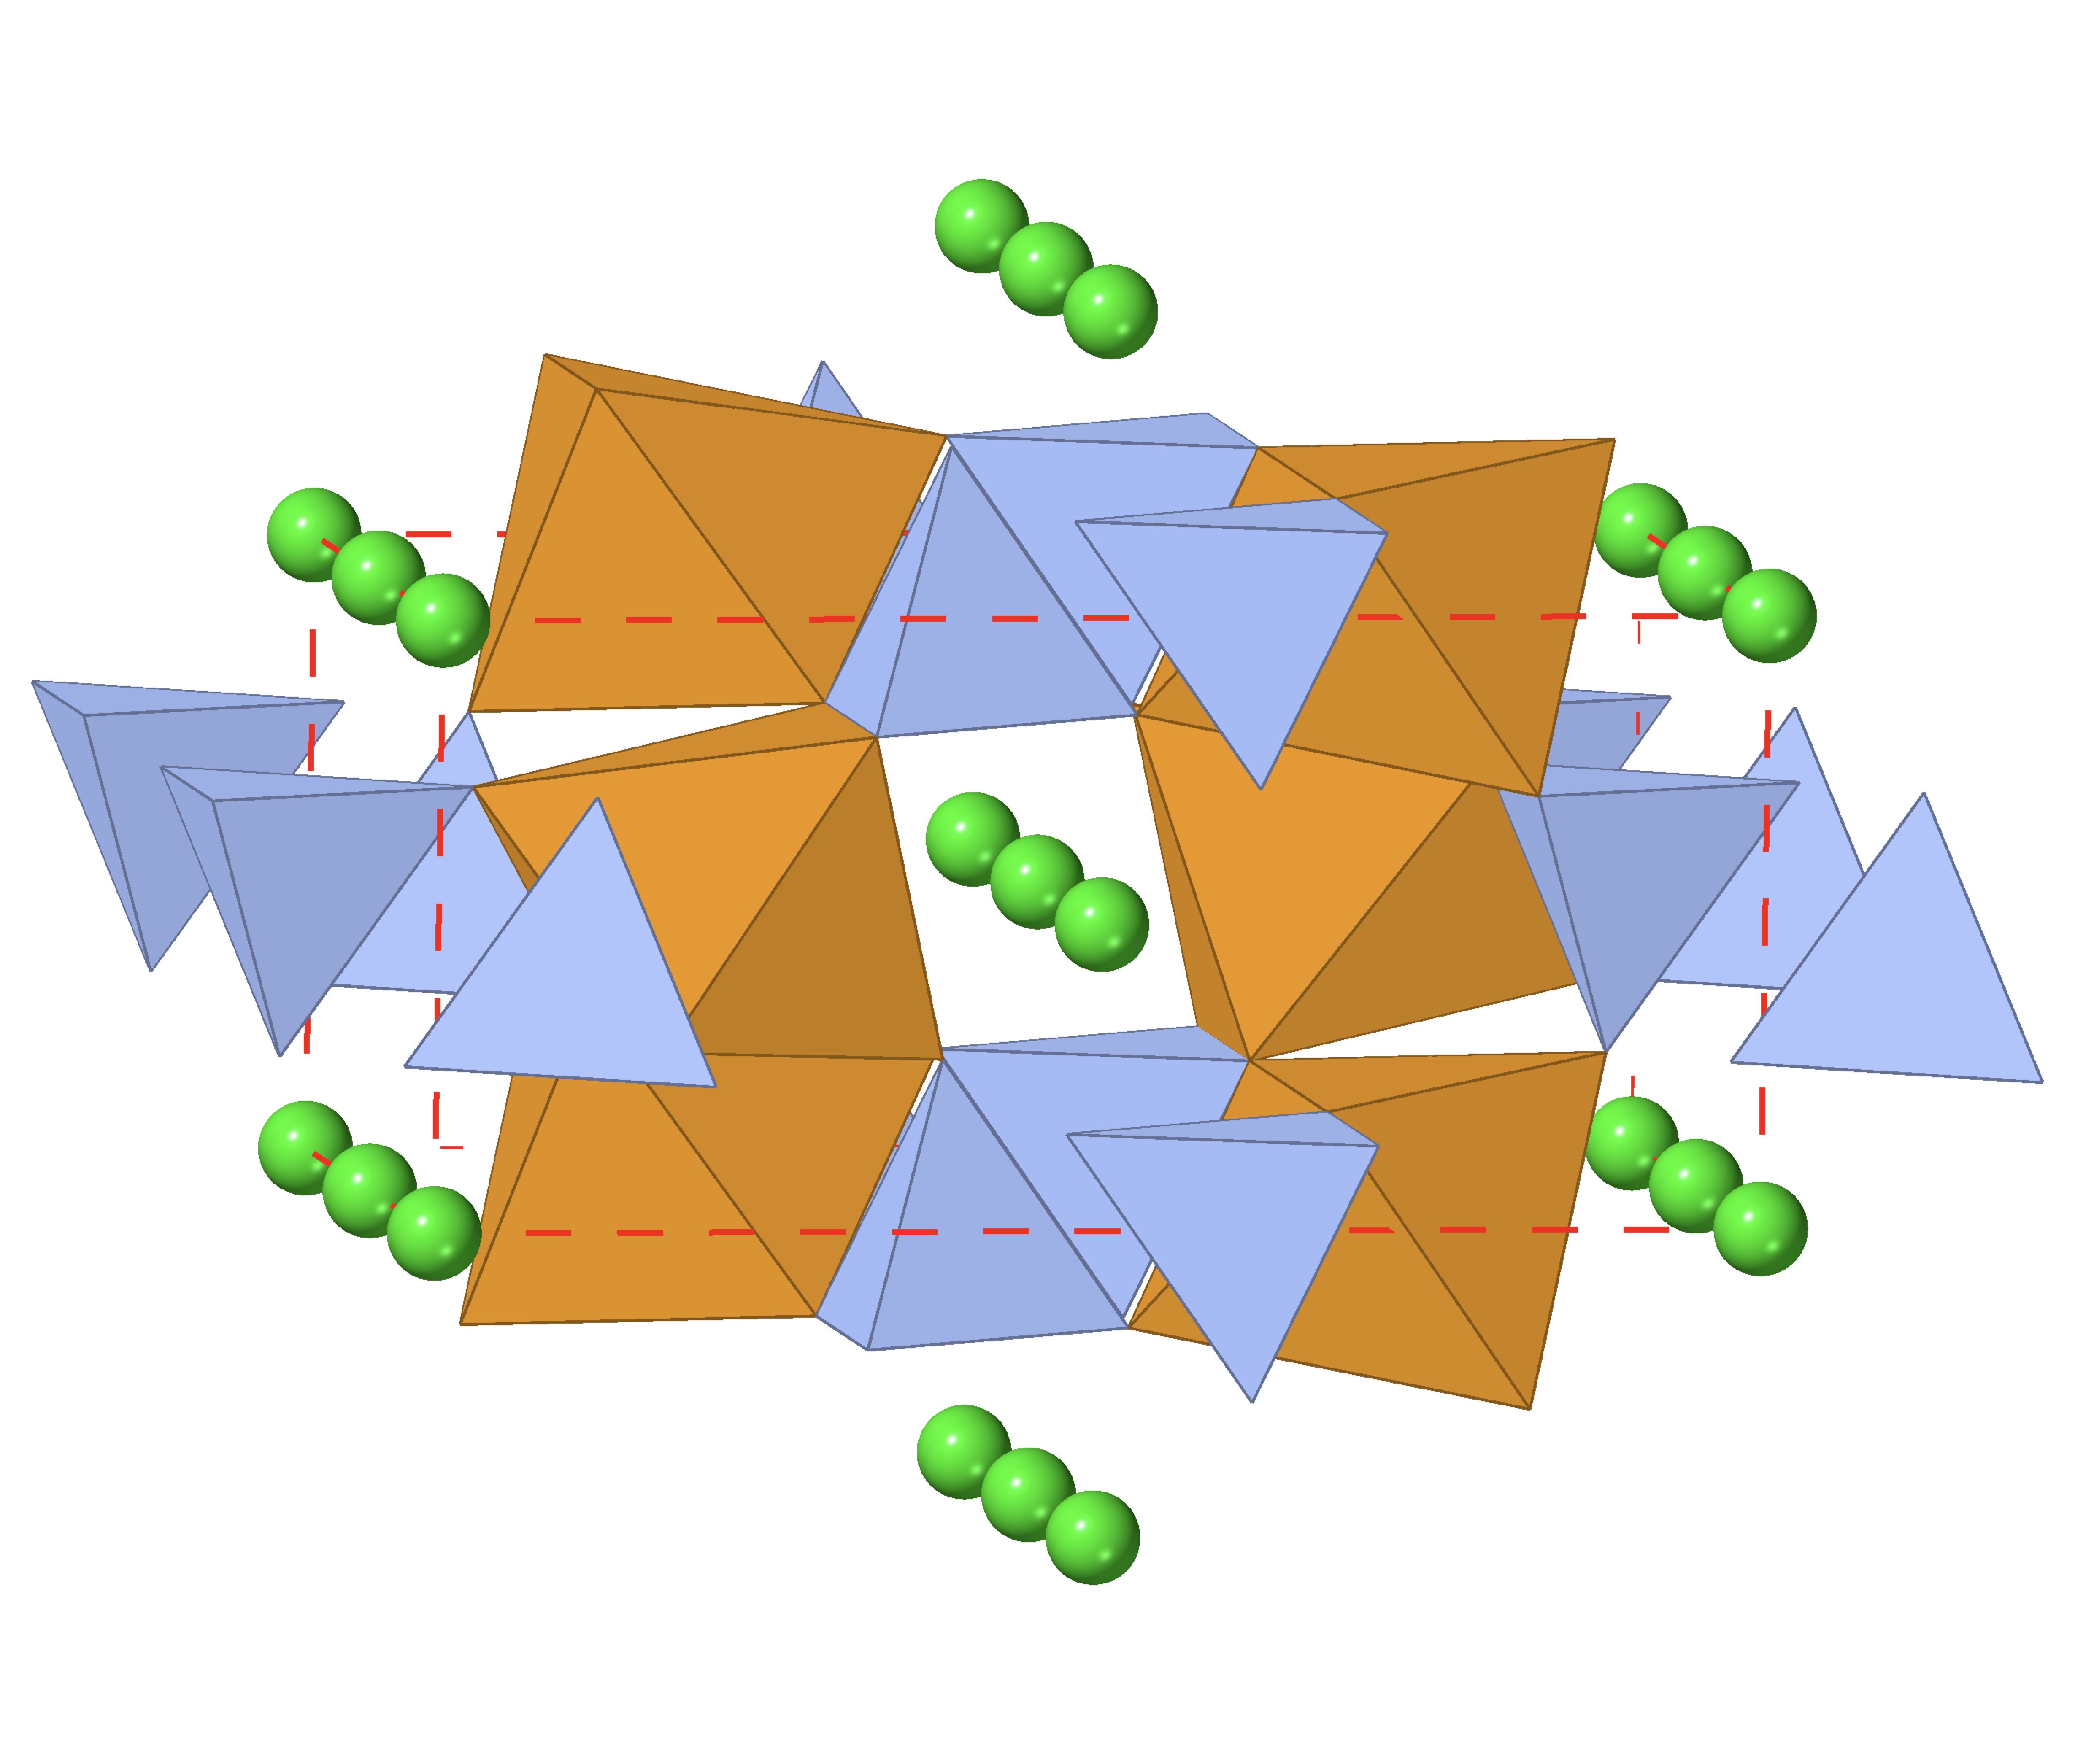
\includegraphics[width=0.6\linewidth]{figures/structures/LiFePO4}

\caption[Olivine-type \ce{LiFePO4}]{Olivine-type \ce{LiFePO4}.  \ce{Li} ions: green; \ce{Fe-O} octohedra: orange; \ce{PO4} tetrahedra: blue.} 
\label{fig:polyanion}
\end{figure}

\subsection{Polyanionic cathodes}
Polyanionic cathodes, derived from the substitution of oxide sites in layered oxides with \ce{(XO_4)^n-}/\ce{(X_mO_{3m+1})^n-} polyanions (X = S, P, Si, As, Mo, W),\cite{Gong2011a} remain of significant research interest.
The strong covalent bonding between these polyanions and \ce{MO_$x$} polyhedra leads to high thermal stability, making these materials suitable for safety critical applications.\cite{Nitta2015}

Goodenough et al.\cite{Padhi1997} initially presented the archetypal polyanionic cathode in 1997, olivine \ce{LiFePO4} (Figure \ref{fig:polyanion}), which remains the only commercialised cathode of this class.
An inductive effect from the \ce{(PO4)^3-} raises the redox potential of the \ce{Fe} centre, yielding a relatively high \ce{Fe^3+/Fe^2+} redox potential of \SI{3.5}{\volt} versus \ce{Li/Li+}, making it suitable for practical applications.
Indeed, this material is commonly used in high power situations, such as power tool applications.
The use of Fe rather than Co significantly reduces material costs, and increases the environmental credentials of this material.

The 1D migration channels\cite{Islam2014} somewhat hinder advancements via metal substitution of this cathode, as those metals with moderate \ce{Li/M} antisite defect concentrations suffer from reduced performance arising due to channel blocking.\cite{Fisher2008b}

\newpage
\begin{figure}
\centering
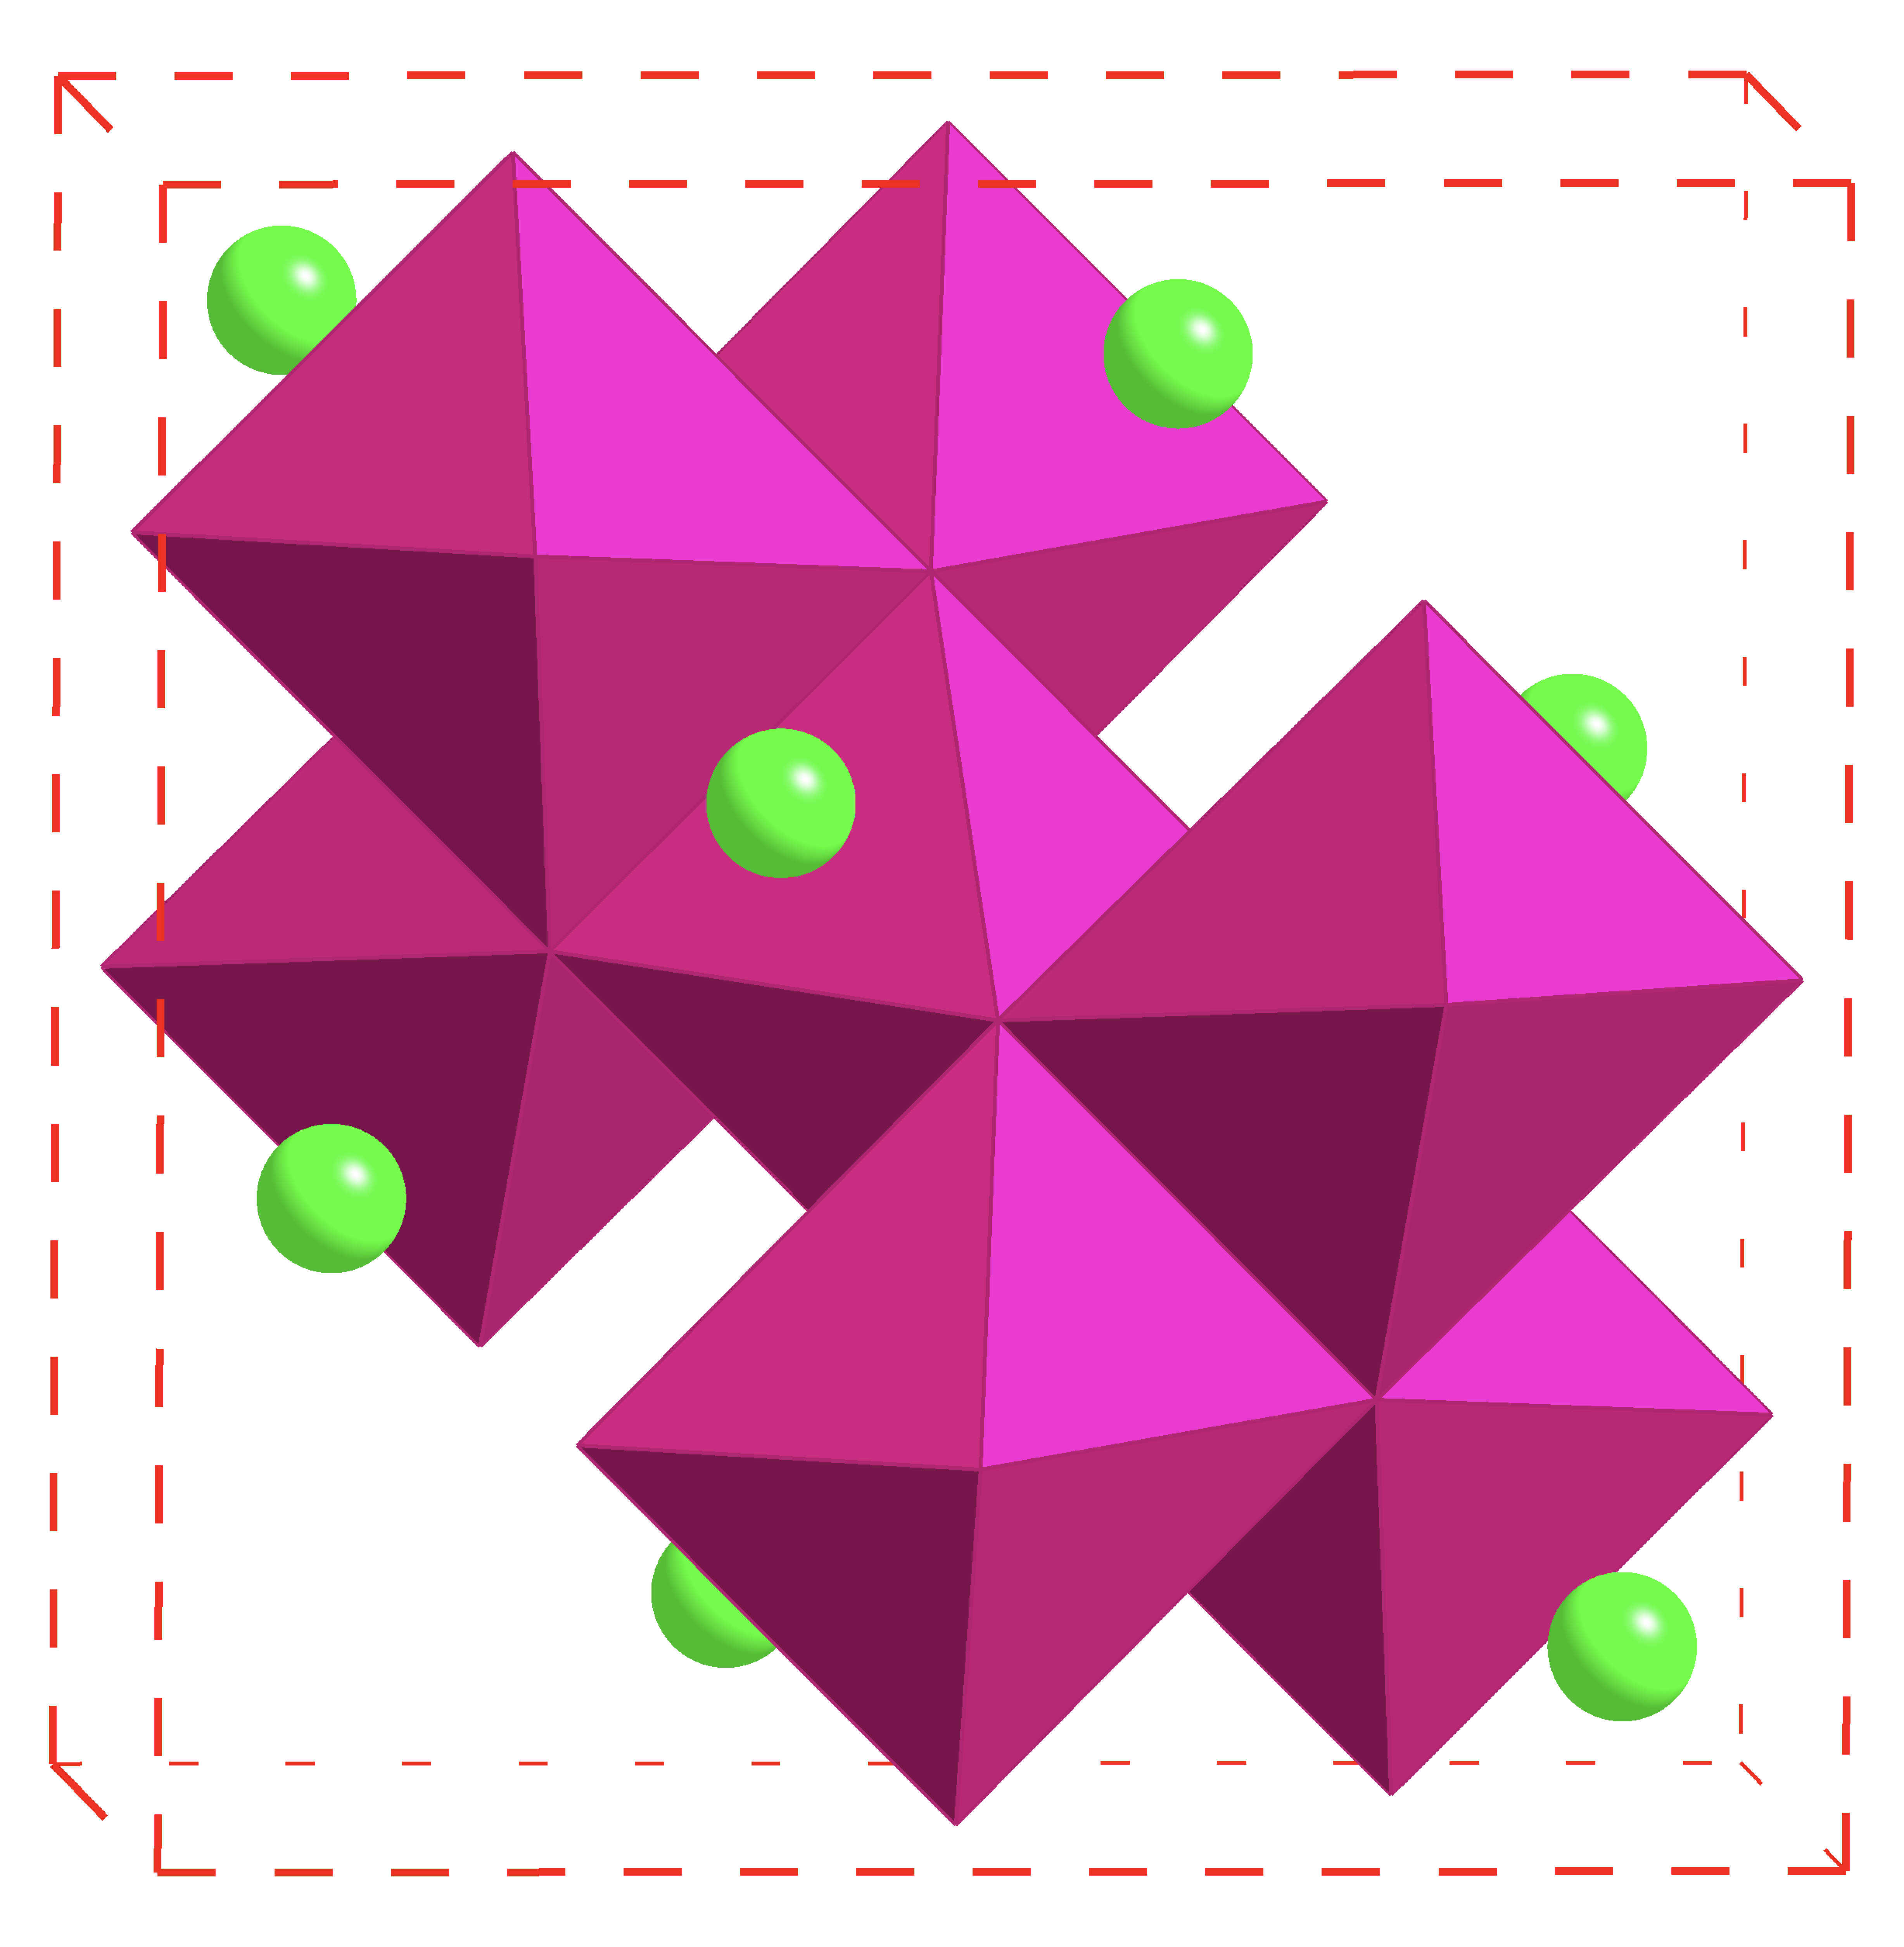
\includegraphics[width=0.7\linewidth]{figures/structures/LiMn2O4}
\caption[Cubic \ce{LiMn2O4} spinel]{Cubic \ce{LiMn2O4} spinel. \ce{Li} ions: green; \ce{MnO6} octohedra: pink.} 
\label{fig:spinel}
\end{figure}

\subsection{\ce{LiMn2O4} spinel (LMO)}
Despite its relatively low capacities (\SI{140}{\milli\ampere\hour\per\gram}), \ce{LiMn2O4} spinel (LMO) has found some commercial success in applications requiring high discharge rates.
Low internal resistance, arising from the 3 dimensional ion conduction pathways, allow for rapid cycling at high currents.

Whilst pure LMO batteries are uncommon, they are commonly coupled with NMC cathodes in EV applications, with the NMC component providing larger capacities, and the LMO component enabling for short periods of high current discharge, as required during rapid acceleration.
This strategy of combining battery chemistries is used in a number of production vehicles including the Nissan Leaf.\cite{Schmuch2018, Blomgren2017}
These cathodes also offer good thermal stability, but have a poor lifespan.
As such, there is interest in phasing out this material to extend the life of new electric vehicles.
\newpage
\section{Li-rich cathodes}
A limitation of the layered oxide materials discussed thus far is the limited extent to which delithiation can reversibly occur.
Even were a means of stabilising these cathodes in a fully delithiated state devised, the theoretical maximum capacities of conventional layered oxide cathodes may be insufficient for future automotive applications.

Li-rich cathodes seek to increase the capacity of conventional \ce{LiMO2} materials by substitution of some portion of \ce{M^3+} for \ce{Li^+}.
The term ``Li-rich'' derives then from the excess of Li relative to transition metals in the cathode:
\begin{equation}
	\frac{[\textrm{Li}]}{[\textrm{TM}]} > 1
\end{equation}

Whilst this does yield higher theoretical capacities due to the increased fraction of Li in the structure, this change also has a potentially negative impact on the electrochemical performance of the cathode:
\begin{labeling}{\textbf{Redox well}}
	\item [\textbf{Stability}] The removal of \ce{M} reduces the number of stabilising \ce{M-O} bonds.
	This reduces the thermal stability and cycle life of the cathodes.
	\item [\textbf{Redox well}] Transition metal species serve to charge compensate the extraction of \ce{Li+} from the cathode.
	Reduced transition metal availability requires other charge compensation mechanisms to allow full extraction of Li.
	\end{labeling}

As Li extraction in excess of one Li per transition metal species has been observed in many Li-rich cathodes, other charge compensation mechanisms must exist.
These mechanisms have been the area of much research, and despite extensive literature on the topic,\cite{Rozier2015,Csernica2019, Li2018a, Seo2016} it remains an area of active debate.
Of particular interest is the O-redox mechanism which has been demonstrated in many systems.\cite{Li2018a}

Whilst many Li-rich materials have been shown to be oxygen-redox-active, they generally exhibit undesirable characteristics including voltage fade, hysteresis, and O loss.\cite{Csernica2019}
The factors which impact these phenomenon have been extensively studied but remain an active and unresolved area of research.\cite{Rozier2015,Csernica2019, Li2018a, Seo2016}
\newpage
\subsection{\ce{Li2MnO3}}
\ce{Li2MnO3}, being an end member of the Li-rich layered oxide cathodes, is one of the most widely studied Li-rich materials.
It exhibits a O3-type monoclinic structure, with an ordered (honeycomb) distribution of \ce{Li+/Mn^4+} ions in the mixed \ce{[Li_{1/3}Mn_{2/3}]O2} layer.\cite{Rozier2015}

Initially thought to be electrochemically inactive due to the already fully oxidised \ce{Mn^4+}, \ce{Li2MnO3} was later shown to  demonstrate a huge theoretical capacity of \SI{285}{\milli\ampere\hour\per\gram}.\cite{Kuganathan2019a}
The electrochemical activity was attributed to a partial loss of \ce{Li2O}, leading to the formation of \ce{Li2MnO3} domains in a \ce{LiMnO2} matrix on partial delithiation.

The use of \ce{Mn} offers huge environmental and economic benefits versus \ce{Co} containing cathodes.
Unfortunately, its poor structural stability during cycling and low electrical conductivity render its use in any practical application infeasible.
It does however provide a relatively simple reference material for study, to allow a better understanding of more complex Li-rich layered oxides.





\begin{figure}
\centering
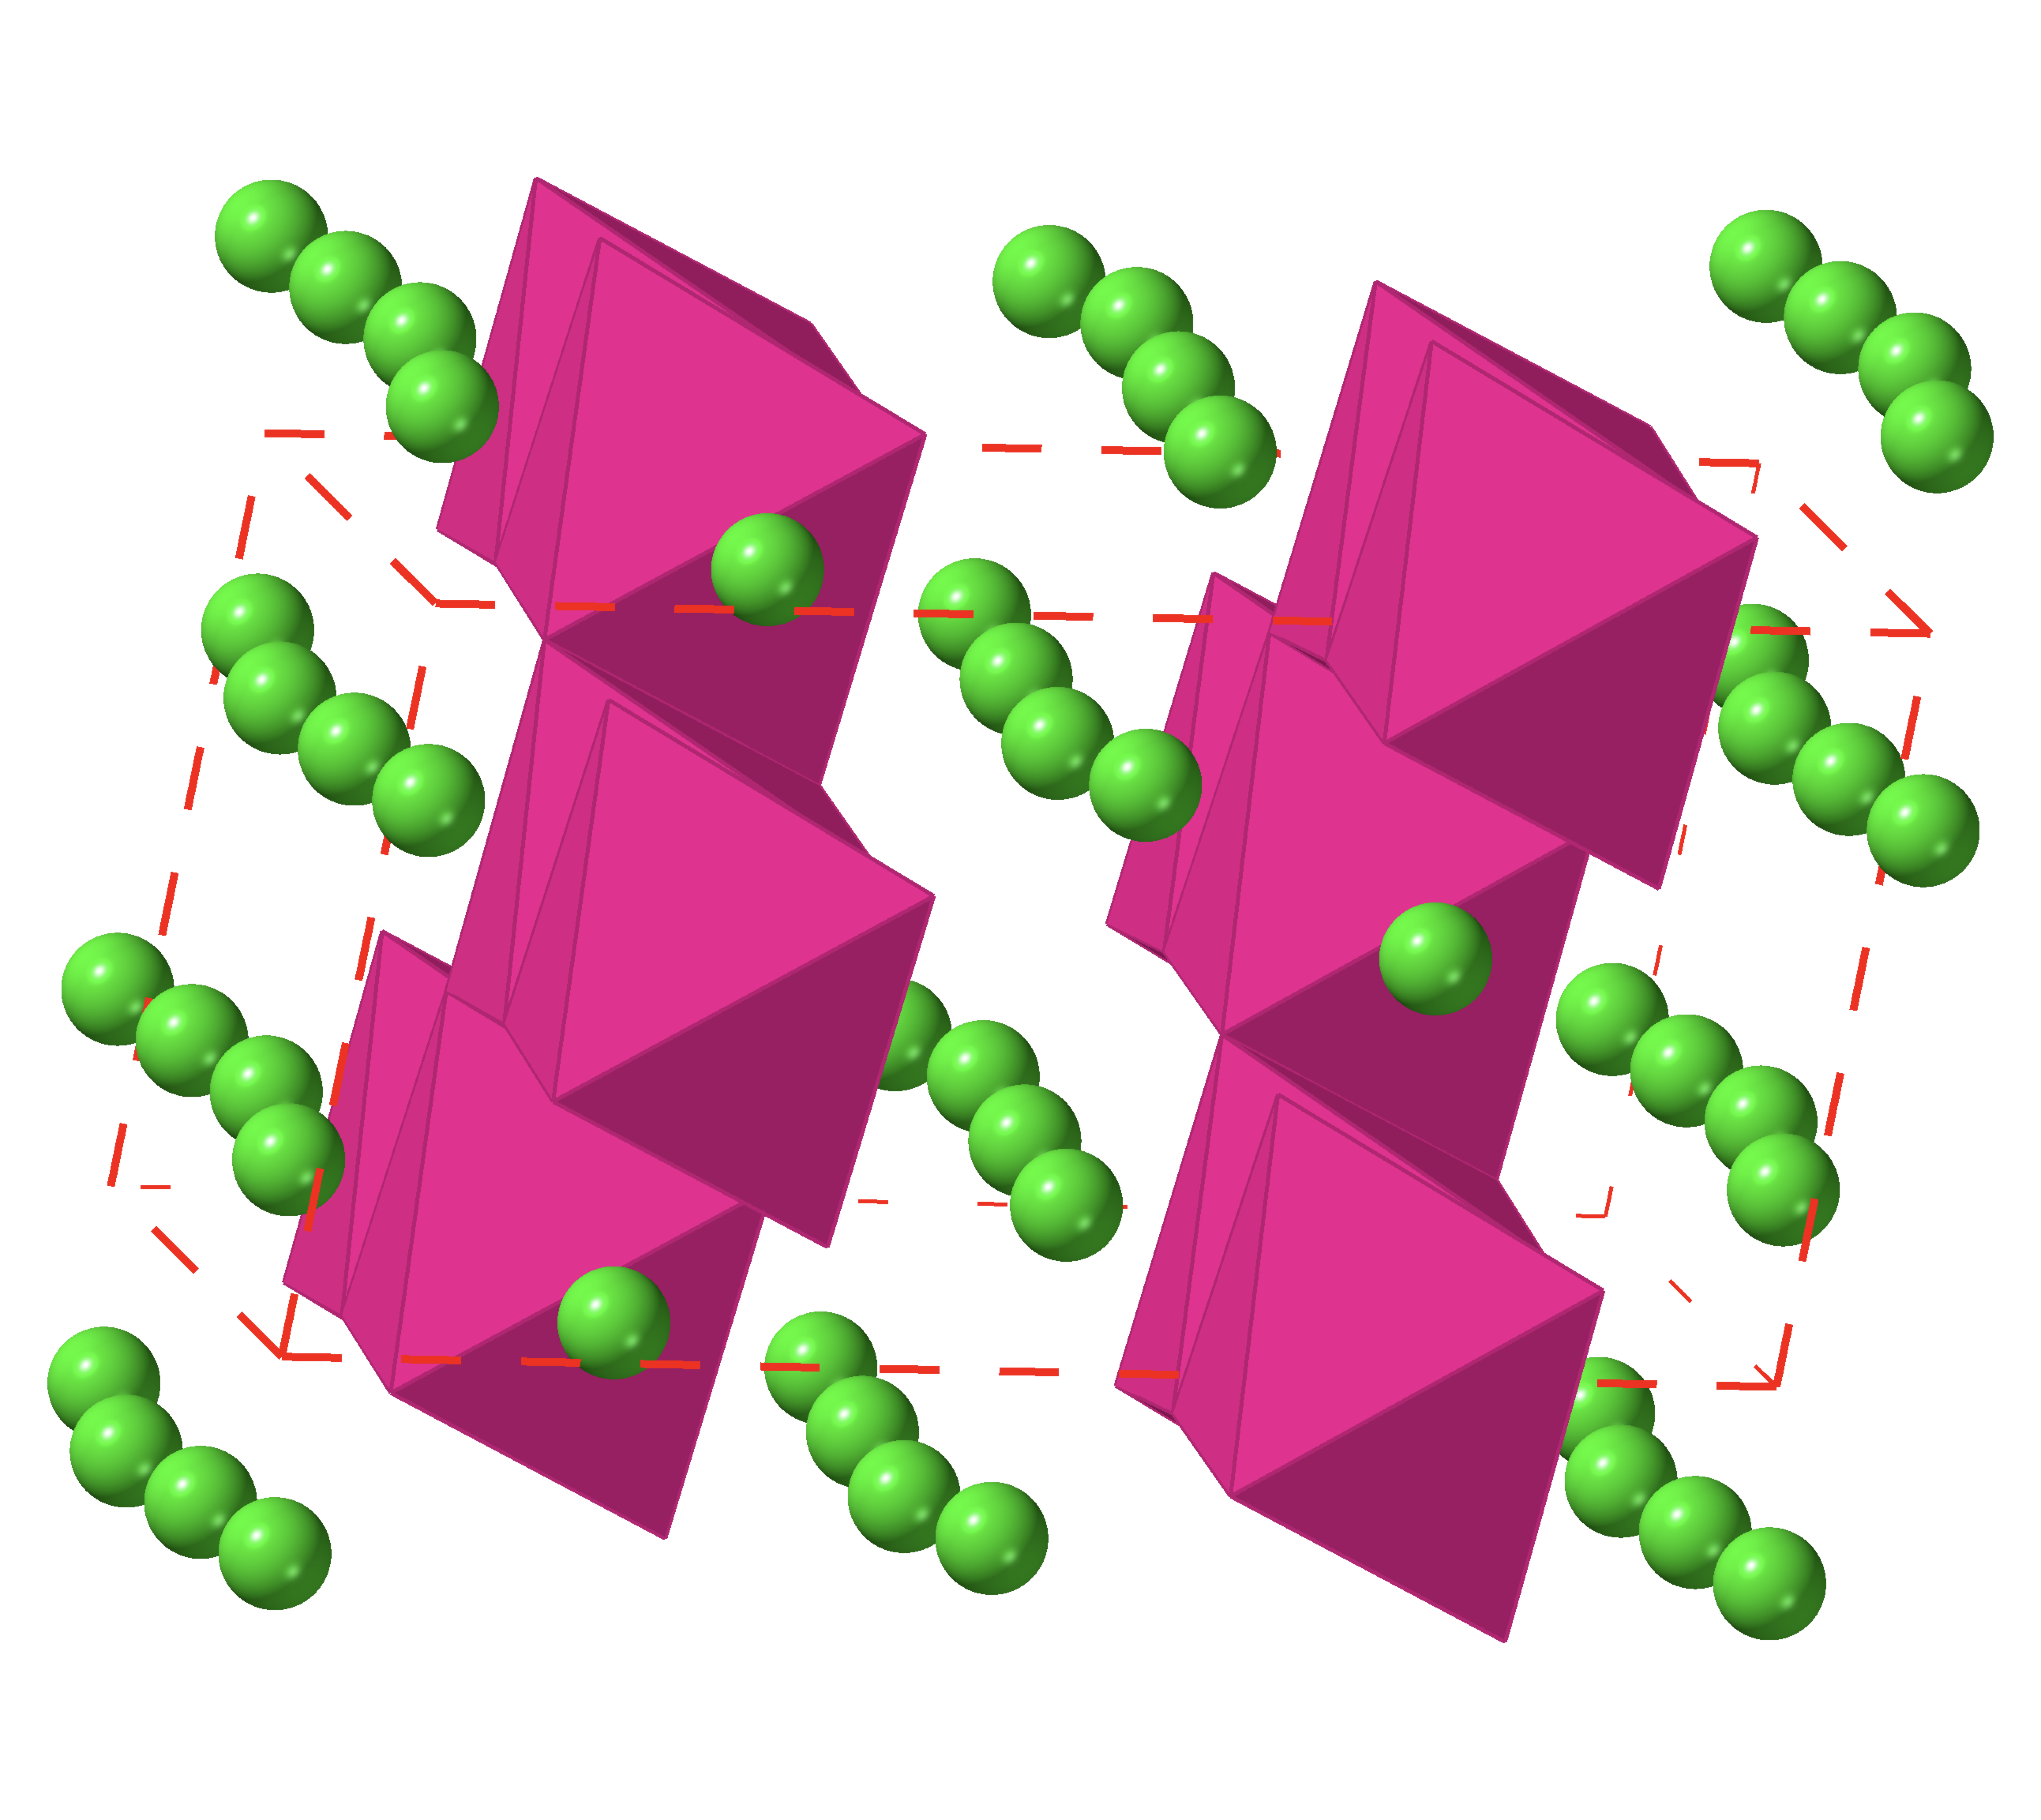
\includegraphics[width=0.6\linewidth]{figures/structures/Li2MnO3}
\caption[\ce{Li2MnO3}]{Layered \ce{Li2MnO3}. \ce{Li} ions: green; \ce{MnO6} octohedra: pink.} 
\label{fig:Li2MnO3}
\end{figure}





\newpage
\subsection{Li-rich NMC}
\begin{figure}
\centering
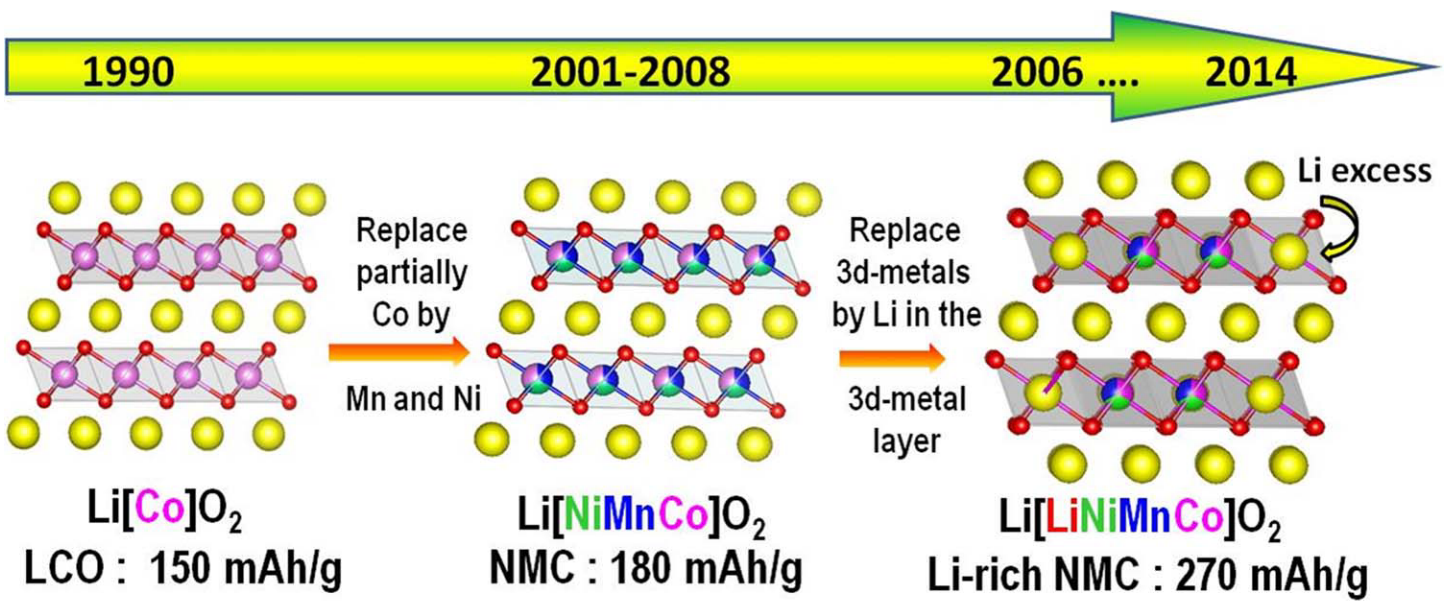
\includegraphics[width=\linewidth]{figures/structures/tarasconNMC}
\caption[Evolution of Li-rich NMC from LCO.]{Evolution of Li-rich NMC from LCO.\cite{Rozier2015}} 
\label{fig:tarasconNMC}
\end{figure}

Li-rich NMC, shown schematically in Figure \ref{fig:tarasconNMC}, is NMC in which some metal species have been exchanged fo Li.
As with the \ce{LiMO2} cathodes, the rich chemistry associated with the presence of multiple metal species offers a wide range of compositions and provides scope to overcome some of the issues associated with the current state of the art Li-rich cathodes, such as voltage fade and O-loss.
Surface coatings have been proposed as a means of extending the lifetime of Li-Rich NMC cathodes, by preventing side reactions with the electrolyte and limiting the formation of non-conductive species which harm electrochemical performance.
Whilst an undeniably useful avenue of research, the additional processing steps may make the implementation of this at a commercial scale infeasible.
Furthermore, the absence of a fundamental understanding of the mechanisms giving rise to these detrimental properties will inevitably hinder progress.
As the exact origin of these phenomenon is not widely agreed upon, and may indeed change between systems, much of the research surrounding Li-rich NMC has been in attempting to better understand the fundamental phenomenon which give rise to these undesirable properties.


\newpage
\subsection{Li-rich disordered rocksalts}
Conventional cathode materials tend to have ordered structures, as the presence of distinct transition metal sites and Li sites/diffusion pathways provides stability upon cycling.
The lack of intermixing of Li and transition metal species is vital to ensure good Li-ion mobility and prevent detriment to electrochemical performance.
Ceder \textit{et al.}\cite{Casimir2014} proposed however, that the ``ordering paradigm'' adopted by the battery community led to a number of viable cathode candidates being overlooked.
By percolation theory, so long as the ratio of Li:TM sites is above some critical concentration, a network of low-energy pathways should exist, allowing mobility and extraction to occur.\cite{Urban2014}

Of particular interest in this work are two disordered rocksalt structures:

\begin{labeling}{\textbf{\ce{Li2MnO2F}}}
\item [\textbf{\ce{Li4Mn2O5}}] First presented in 2015 by Freire \textit{et al.},\cite{Freire2016} this material demonstrates a huge specific capacity of \SI{355}{\milli\ampere\hour\per\gram}.
Diaz-Lopez \textit{et al.}\cite{Diaz-Lopez2018} characterised the material, demonstrating that a \ce{MnO} rocksalt structure with high \ce{Li/Mn} disorder at cationic sites, and 1/\nth{6} O vacancies at the anionic site provided good agreement with synchrotron and powder diffraction data.
Yao \textit{et al.}\cite{Diaz-Lopez2017}, and later Bhattacharya \textit{et al.}, used these findings as a basis for a DFT study.
These studies identified a number of ordered structures which were of a lower energy than quasi-disordered structures.

\item [\textbf{\ce{Li2MnO2F}}] Initially presented in 2018 by Bruce \textit{et al.},\cite{House2018} \ce{Li2MnO2F} also exhibits disorder on both the cation and anion sites.
With a discharge capacity of \SI{280}{\milli\ampere\hour\per\gram}, half of which arises from O-redox, the material is both an interesting candidate to better understand the anion redox processes exhibited in other Li-rich cathodes, and an excellent cathode candidate itself.
Furthermore, there is little evidence of O-loss, distinguishing it from layered Li-rich cathodes.
There is currently no literature beyond the paper in which the material was initially presented. 
Dr Ryan Sharpe, in collaboration with the author, is currently preparing a manuscript pertaining to a DFT study of this material.
\end{labeling}

\section{Project aims and chronology}
Whilst both \ce{Li4Mn2O5} and \ce{Li2MnO2F} have been studied with DFT, either in literature or in preparation, there have thus far been no defect or dynamic computational studies of either material.
This information may be key to understanding the role of local ordering on electrochemical performance, and may inform future experimental work.
As such, this work contains atomistic studies of each of these materials, focusing particularly on properties of interest for battery materials.

It is worth clarifying at this point that the trivial tone in which the above problem is stated in no way correlates with the difficulty of the task!
Much of the work done in the past year has focused on methods development, as the disordered nature of these materials demands the use of interatomic potentials which are stable for a wide range of local environments.
Furthermore, random structure generation lends itself to the creation of unphysical local environments by the law of large numbers if not biased against.
Whilst readily handled in DFT, where the first principles nature of the calculations lend themselves well to handling a wide range of states, interatomic potentials are generally derived to describe a particular system.
Disordered systems, with more local environments than conventional ordered materials, give rise to a number of issues in atomistic simulations.

\ce{Li2MnO2F} was the first material studied in this project. 
The difficulties in obtaining reasonable results were attributed not to the disorder in the system, but to the lack of a suitable Mn-F potential in literature.
It was only when similar issues manifested in the \ce{Li4Mn2O5} system that the disorder was identified as the source of difficulty. 


\chapter{Computational methods}
\section{Introduction} % TODO Update from MRes version
Computational techniques are a vital tool in the prediction and characterisation of solid state materials.
Not only can computational methods reduce experimental load by identifying promising material candidates in screening studies, but they can offer atomic scale insights into the structural and transport properties of materials not observable by experiment.

This study primarily uses potentials-based minimisation techniques and Molecular Dynamics (MD), implemented in GULP \cite{Gale2003} and LAMMPS \cite{StevePlimton1995} respectively.
In this chapter, the fundamental concepts and mathematics underpinning these techniques are presented.
Furthermore, an overview of classical interatomic potential fitting strategies are presented and contrasted with in development techniques.to contrast to the work presented herein. %TODO chapter reference
This overview is brief and focuses primarily on techniques used in this report, as more comprehensive reviews are available elsewhere. \cite{Gale2003, Jensen2007, Catlow2013}
Some work presented in this section is derived from the MRes report which led to this project, as the fundamental equations underpinning computational methods remain the same.

\section{Atomistic modelling}
An understanding of the forces atoms experience as a function of their environment is vital to gain insights into the properties of systems of interest.
One class of approaches for calculating the interatomic forces between atoms, \textit{ab initio} techniques, are based on quantum mechanics, and seek to determine electron density as a function of position. Whilst the scale of systems these strategies can be used for is increasing with developments in computational resource available, these techniques remain prohibitively expensive for large systems or systems studied over large time-scales.

In contrast, atomistic techniques seek to express the forces between atoms as a series of empirically derived models, either fitted to experimental or \textit{ab initio} data, which can be cheaply evaluated, allowing for large scale systems to be studied over large time scales. This is particularly important when considering phenomenon which occur over large time scales, such as diffusion. 

\section{Potential models}
All atoms in a system, and their current position, momentum, and oxidation state, give rise to highly complex interactions contributing to the internal energy of the system, which must be enumerated if a perfect atomistic model is to be developed.

Potential models are used to determine the forces in such systems by treating these as a series of discrete isolated interactions which sum to the same overall effect. 
The internal energy of the system can then be given as the sum from one to n-body terms as such:\cite{Gale2003}
\begin{align}
U &=& &\sum_{i = 1} U_i&         &+& &\frac{1}{2}\sum_{i = 1} \sum_{j = 1} U_{ij}&  &+& &\frac{1}{6}\sum_{i = 1} \sum_{j = 1} \sum_{k = 1} U_{ijk}& &+& &\cdots\\
&=& &\sum_{i = 1}^\prime U_i&  &+& &\sum_{i,j = 1}^\prime U_{ij}&                 &+& &\sum_{i,j,k = 1}^\prime U_{ijk}&                           &+& &\cdots
\label{eq:taylor}
\end{align}
With the first term accounting for single-body terms, the second term accounting for those interactions which exist between pairs of bodies and so on.
The primed sum in Equation \ref{eq:taylor} distinguishes between interactions that are enumerated repeatedly, and instead counts each unique interaction only once, hence cancelling the $\frac{1}{N!}$ term.
This expansion is exact if expanded to account for all N-body interactions in a system.

As it is only the low order terms which give rise to the majority of the internal energy of a system, it suffices to truncate this expansion to lower order terms.
Typically, this is limited to two-body terms, although higher order terms are included where these strongly impact the system (e.g. bond angles).
Beyond this, higher order terms are only considered where the calculation of a specific property of interest requires their inclusion.
Three-body interactions are required to calculate phonon distribution curves for example.

Furthermore, as the number of bodies in an interaction increases, it becomes increasingly difficult to find a rational physical basis on which an empirical model can be based. 
 
Single body interactions are implemented to represent an external forcefield being applied to a system, such as the application of an external electric field interacting with charged species.
They are also used in the Einstein model, in which species do not interact with one another, and instead are attached to their lattice sites by a spring term.
Single body terms are not used in the course of this study, but are referenced here for completeness sake.
\subsection{Two-body interactions}
The two-body terms in Equation \ref{eq:taylor}: 
\begin{equation}
\sum_{i,j = 1}^\prime U_{ij}
\end{equation}
account for the interactions occurring between pairs of atoms or ions in isolation.
As no reference frame is given, these terms are therefore strictly a function of interatomic separation.
It is conventional to further subdivide these two-body interactions into Coulombic (long-range) and short-range terms as so:
\begin{equation}
U_{ij} = \Phi_{Coulombic} + \Phi_{short-range}
\label{eq:two-body}
\end{equation}

The Coulombic term in Equation \ref{eq:two-body} is the potential arising from electrostatic interactions between pairs of charged species:

\begin{equation}
\Phi_{Coulombic} = \frac{q_iq_j}{r_{ij}}
\label{eq:coulombic}
\end{equation}
Where $q_i$ and $q_j$ are the effective charges of the species.
This term is colloquially referred to as the ``long-range'' term, as the non-Coulombic component of these interactions are comparatively tiny beyond a certain range.
It is also typically the dominant component in a system at equilibrium, accounting for around 90\% of the total potential energy in a usual system.\cite{Catlow2013}

The long-range nature of the Coulombic term leads to slow convergence in direct space for a large number of ions.
The \citet{Ewald1921} summation can be used to overcome this shortcoming in periodic systems, by further subdividing the Coulombic interactions into short- and long-range terms.
The short-range components are computed as before, while the long-range terms are solved in reciprocal space.

The nature of a two-body interaction can vary widely dependent on context, with the species, charge, and even local environment impacting the resultant potential.
Depending on the system, covalent interactions, London interactions and electron-pair repulsions may all need to be accounted for with no actual calculation of electron density occurring on which to base the potential.

This can include electron-pair repulsions, London interactions and covalent interactions.
This term can be calculated through the use of tabulated data, or via simple analytical models.
Analytical models are typically empirically derived from experimental data.

The selection of an appropriate model is vital, with considerations including the ionic/covalent nature of the system, availability of experimental data, and computational cost influencing the choice of model.
Furthermore, given potential models are often derived to match experimental data for a given system, ensuring that that same potential is suitable when applied outside of the context in which it was developed is important.

This of course can pose an issue when seeking to study systems where no experimental data is available with which to verify the findings of computational work.
 For ionic systems, the Buckingham Potential form is conventionally used to for two-body interactions:


\begin{equation}
\Phi_{ij} = A\cdot \exp \left(\frac{-r_{ij}}{\rho_{ij}} \right) - \frac{C}{r_{ij}^6}
\label{eq:Buckingham}
\end{equation}

\noindent Other common short range potential models are given in Table \ref{tab:potentialmodels}

\begin{table}[t]
  \centering
  \caption{Common short-range two-body potential models.\cite{Gale2003}}
  \label{tab:potentialmodels}
  \begin{tabular}{@{}lc@{}}
  \toprule
  Potential Model         & Expression     \\
  \midrule
  Buckingham              & $\displaystyle{\Phi_{ij} = A\cdot \exp \left(\frac{-r_{ij}}{\rho_{ij}} \right) - \frac{C}{r_{ij}^6}}$    \\
  \addlinespace
  Harmonic                & $\displaystyle{\Phi_{ij} = \frac{1}{2}k_2(r_{ij}-r_0)^2   + \frac{1}{6}k_3(r_{ij}-r_0)^3    + \frac{1}{24}k_4(r_{ij}-r_0)^4   }$    \\
  \addlinespace
  Lennard-Jones           & $\displaystyle{\Phi_{ij} = \left(\frac{A}{r_{ij}^m} \right) - \left( \frac{B}{r_{ij}^n}\right)}$   \\
  \addlinespace
  Morse                   & $\displaystyle{\Phi_{ij} = D_e \left((1- \exp(-a(r_{ij} - r_0)))^2           -1\right) }$    \\
  \bottomrule
  \end{tabular}
\end{table}

\vspace{-5pt}
\paragraph{Finite-range implementation}
As the name suggests, the short-range terms dominate in the short-range, but the force arising from these interactions decreases rapidly with increasing interatomic distance.
To decrease the computational expense, a threshold radius is defined beyond which all forces are assumed to be zero.
The selection of this threshold is important, as the computational expense is of $O(r_t^2)$, so the shorter this radius the less expensive the simulation, whereas too small a radius will result in a change in the simulation result and decrease in model quality.

In order to prevent this strategy introducing discontinuity into the system, additional terms are added to smoothly reduce the interatomic potential and associated energy derivatives to zero at the threshold radius. %TODO rephrase


\subsection{Three-body interactions}
The nature of three-body terms are dependant on the interactions between three ions or atoms.
These can be interpreted as bond pair repulsions or as a charge dispersion between three bodies in covalent and ionic interpretations respectively.
This term is small relative to the two-body terms, and is usually only included when high degrees of accuracy are required, or for the calculation of properties dependent on three-body interactions such as phonon distribution curves.

A commonly used three-body potential is the harmonic model:
\begin{equation}
  U_{ijk} = \frac{1}{2}k_2(\theta-\theta_0)^2   + \frac{1}{6}k_3(\theta-\theta_0)^3    + \frac{1}{24}k_4(\theta-\theta_0)^4
  \label{eq:threebody}
\end{equation}

In this model, an equilibrium angle is assigned to a bond pair, and any deviations from this angle increase the potential energy of the system.

\subsection{Polarizability}
The electron distribution surrounding an atom or ion will shift according to the local environment in which it exists, effectively allowing the internuclear and electronic interactions to partially decouple.
A rigid ion model, in which species are modelled as point charges, does not capture this behaviour, defreasing the accuracy of models using it.
This is a particularly important behaviour when studying ion migration, and so a failure to account for this behaviour can negatively impact the accuracy of results obtained.

An early model of ion polarisation is the point polarisable ion model (PPI), in which the dipole moment of an ion ($\mu$) is directly proportional to the strength of the electric field in which it sits (E):
\begin{equation}
\mu = \alpha E
\end{equation}
Whilst computationally inexpensive and easily extensible to higher order polarizabilities (i.e. quadrupolar systems), this model performs poorly when handling dynamic lattice properties.
It also poorly predicts dielectric constants, which is easily measurable experimentally and thus a useful criteria for model validation.

This shortcoming can be rationalised by the failure to account for the polarisation of adjacent ions, that is, that neighbouring species being polarised impacts the local electric field and serves to dampen polarisation overall.
Consequently, this model tends to overestimate dielectric constants if tuned to accurately predict another physical property (e.g. elastic constants).


\begin{figure}[ht]
  \centering
  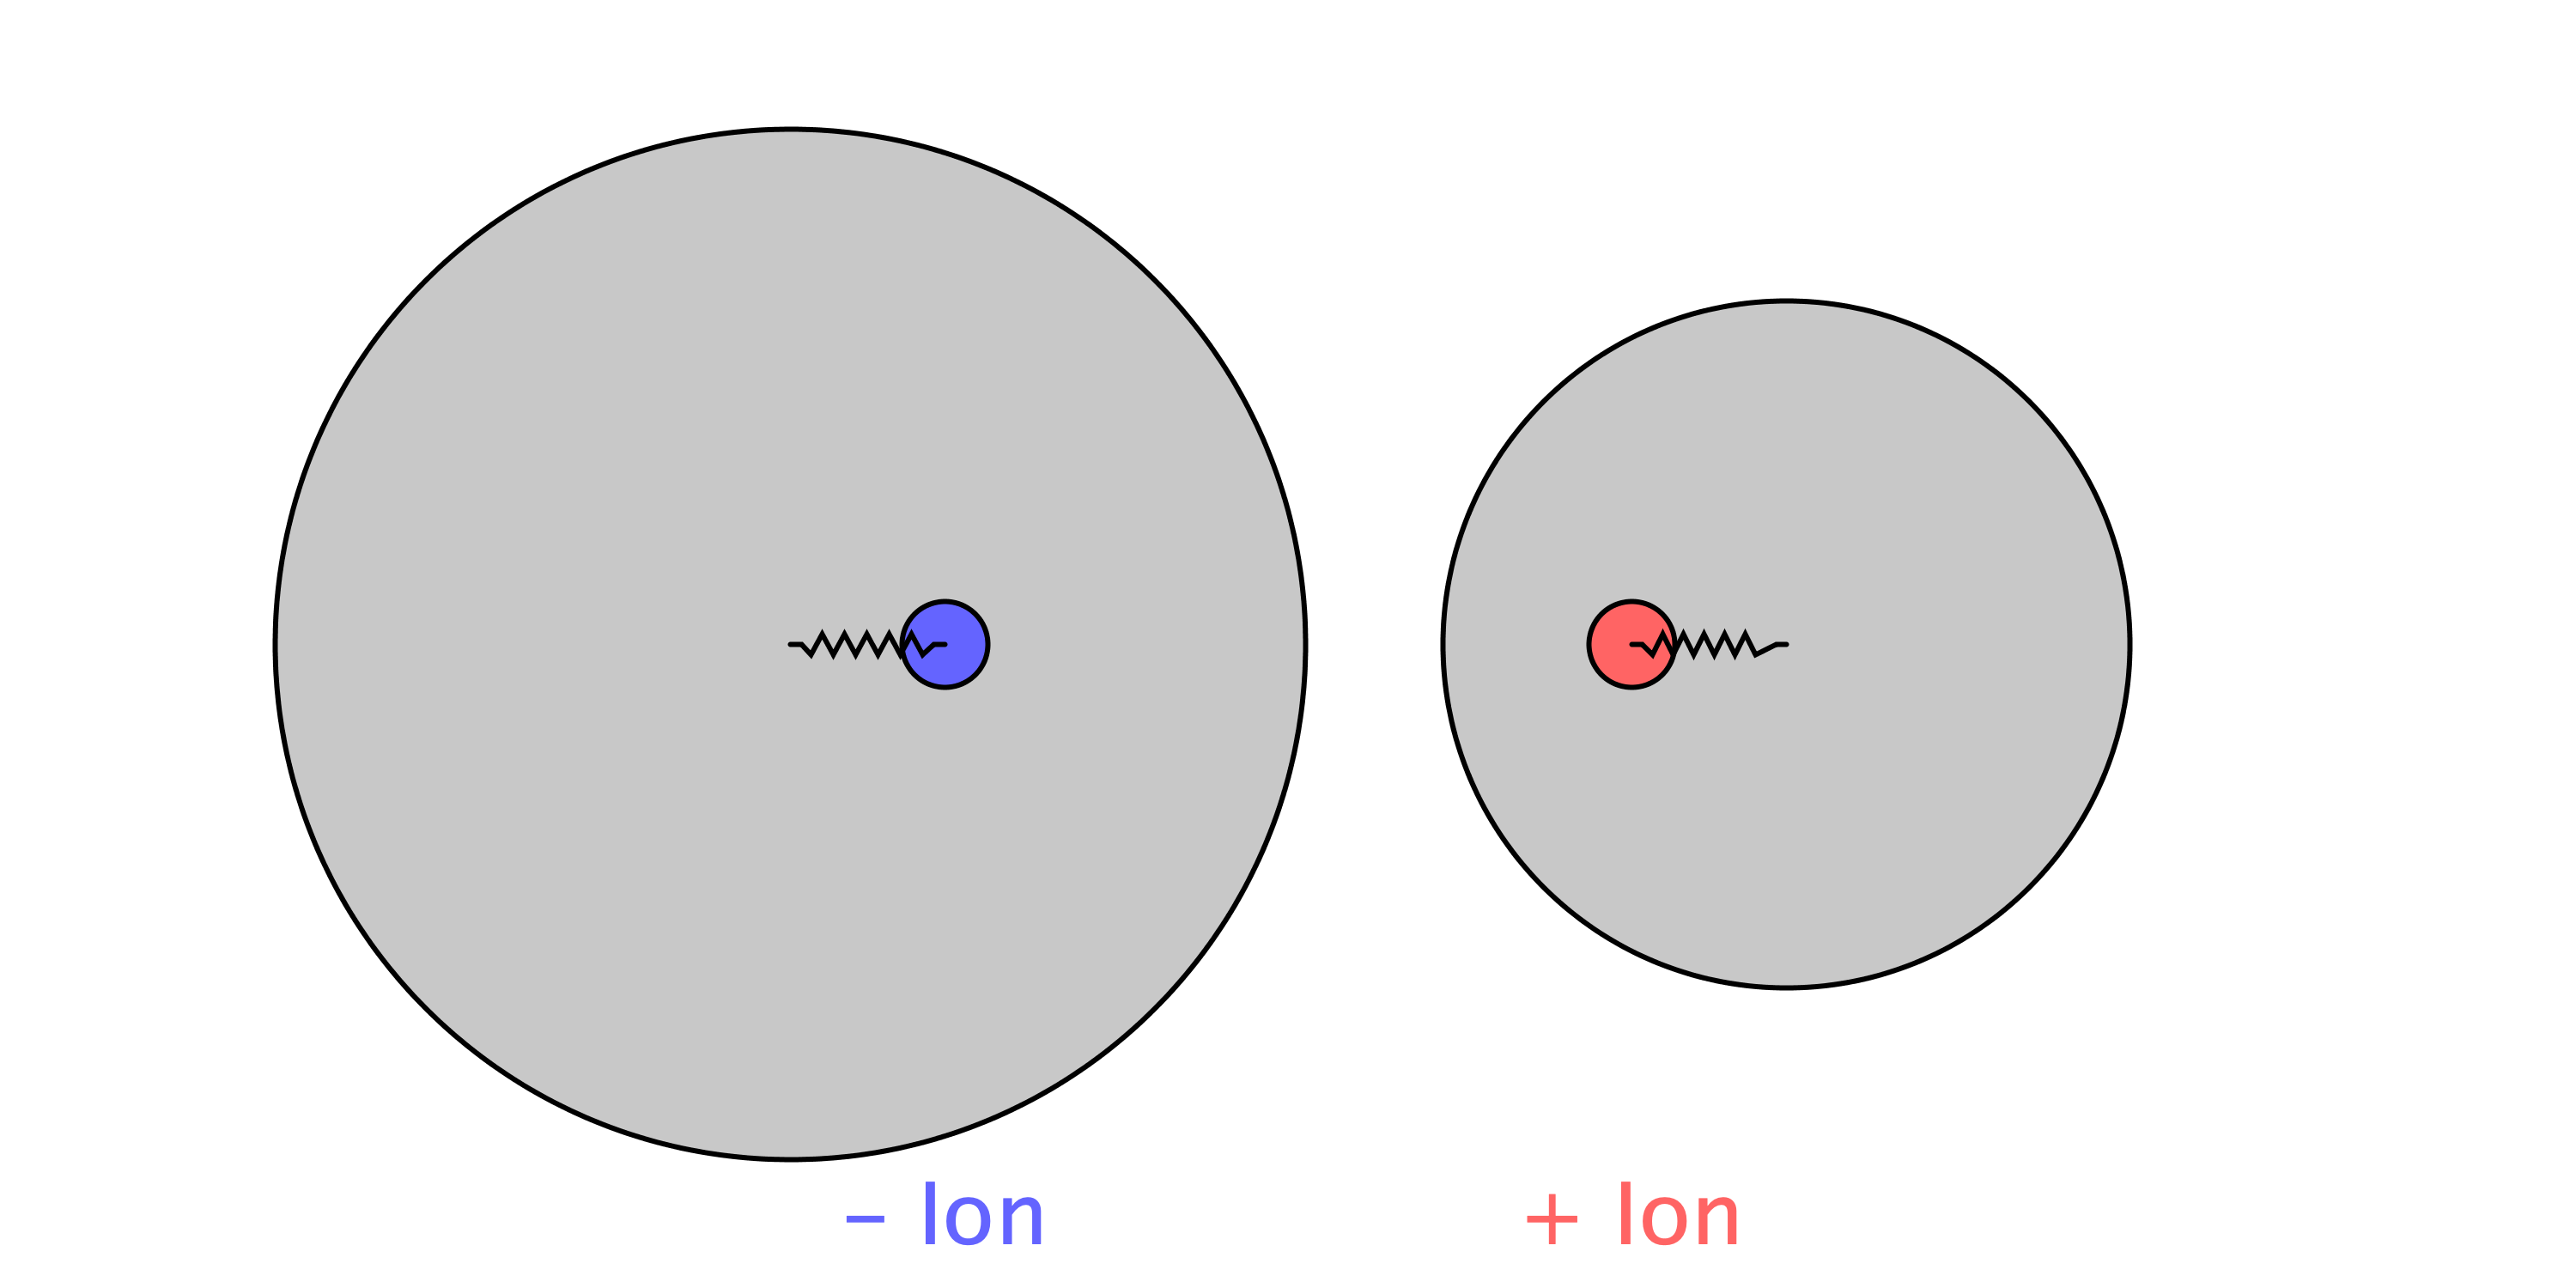
\includegraphics[width=\linewidth]{figures/coreshell/coreshell}
  \caption[Shell model schematic]{Schematic of the shell model of polarisability. The valence electron shells (grey) are attached to the ion core by a harmonic spring, and are displaced by nearby charged species or net electric fields.}
\end{figure}
The shell model\cite{Dick1958} is another computationally inexpensive model of polarisation which accounts for polarisation coupling, thus overcoming a key limitation of the PPI model.
Polarisation coupling is modelled by treating the valence electron cloud as a shell connected to the ionic core by a harmonic spring.
The core represents the nucleus and core electrons of the ion, accounting for the majority of the mass of the ion, while the shell is represents the polarisable valence electrons.
The mass of the shell is treated as zero in non-dynamical systems (i.e. in structural optimisation, Section \ref{sec:minimization}) where the solver strategies are able to handle zero-mass species without instability.
In the case of dynamic systems (i.e. Molecular dynamics, Section \ref{sec:MD}), the shell is assigned a small portion of the overall mass to provide a degree of inertia and remove the need for prohibitively small time-steps.

By allowing the displacement of valence electrons from the ion core, an effective dampening of the polarisation occurs, offering better agreement with experiment.

The charges assigned to the core and shell respectively must sum to that of the point charge it replaces, but the values of these and the spring constant are typically empirically derived.
This polarisation model generally gives good agreement with experiment for ionic halides and oxides.

\section{Partial occupancy and disorder}
Partially occupied sites are those which have no fixed species occupying them, but instead contain vacancies, or some species in a known ratio when summed throughout the whole material.
Disordered solids contain partially occupied lattice sites where the species (or lack thereof) shows no regular ordering in space, instead being randomly distributed throughout the material.



One strategy for addressing this is to use the mean-field approximation. 
At each partially occupied site, the interatomic potentials are calculated as usual for each species which occupies the site. 
The forces are then scaled according to the relative occupancy of each species:

$$
U_{ij} = o_io_jU_{ij}
$$

The sum of these scaled potentials yields the mean potential arising from the partially occupied site.
This technique can be powerful for initial studies of systems in that it yields symmetric (and thus robust) systems, and bypasses the cost issues arising from the combinatorics of generating large systems capturing all likely local environment.
It is particularly useful for the calculation of structural properties, where the averaging of forces is in effect done when determining large scale parameters.

That said, the simplification of lattice sites fails to capture the nuance of local environments, potentially missing properties that might only arise in environments containing certain configurations of species.
As such, caution should be exercised when applying this technique to calculate diffusion barriers.
Furthermore, the implementation of this technique is poorly compatible with the core-shell model in GULP, preventing their simultaneous usage.

Another strategy for handling partially occupied and disordered systems is the supercell approach.
The primitive cell is expanded to be repeated a given number of times in the direction of each basis vector, yielding a supercell.
Each partially occupied site is then assigned one of the species potentially occupying it, such that the desired stoichiometry is achieved across the whole supercell.

Assigning these sites it itself a problem to which many strategies can be applied.
The brute force approach of testing all configurations in not viable for all but the simplest of systems due to the combinatorial nature of the problem.
A simple example of distributing 50 ions and 50 vacancies across 100 symmetry inequivalent sites yields $\frac{100!}{50!\cdot50!} = 10^{29}$ distinct cases.

Another strategy is to randomly assign a species to each site, weighted by stoichiometry.
It is worth clarifying that while perfect disordering is possible, the energetics associated with the formation of a given local environment may bias such systems to exhibit certain local configurations preferentially.
As an example, a disordered rocksalt with a small portion of vacancies at the anionic site might na{\"i}vely be expected, in a sufficiently large system, to have some cationic sites surrounded by six vacancies.
However, the energetics associated with the formation of this local environment would significantly reduce the likelihood of its formation.

Accounting for this when attempting to generate disordered supercells is non-trivial, as the energetics of the environment are not known ahead of time, and the law of large numbers dictates that these sites will form if not biased against.
Further, the potential models used may not be suitable for modelling such unfavourable environments.
Indeed, this problem becomes even more challenging when seeking to derive potentials to fit a disordered system, as the potentials are needed in order to calculate the energetics of the local environments, yielding a {\color{red} chicken and egg type} issue.

A final strategy is to approximate the disordered solid as being ordered.
A benefit of this strategy is it can be coupled with DFT studies to predict low energy ordered structures as a basis for the calculation.
Further, this technique typically yields smaller supercells, making studies in GULP (where periodicity can be leveraged to speed up calculations) significantly cheaper.
Finally, the increased symmetry and reduced number of local environments present makes finding a robust set of potentials easier for such systems.

This of course relies upon a means of generating a low energy or ground state structure for the system being studied, which is itself a non-trivial matter.
One such strategy, cluster expansion, \cite{Bhandari2019} was utilised by the authors of source material for this report, and may be implemented by the author in future work.


\section{Energy minimisation}
\label{sec:minimization}
\subsection{The configuration space}
\label{sec:config}
The internal energy of an ionic system is a function of its atomic coordinates.
While such systems are more easily thought of as a series of points in a 3-space, the resultant energy surface is $3n$ dimensional for a system containing $n$ atoms, with each point on this surface corresponding to a unique set of atomic coordinates.
We define the vector of positions of these atoms, the configuration space, $\mathbf{x}$.

Whilst each position in the configuration space has an associated energy, $U(\mathbf{x})$, real systems tend towards more energetically favourable states.
Stationary points on the energy surface, those where $\nabla U(\mathbf{x}) = 0$, are of particular interest:
\begin{labeling}{\textbf{Saddle point}}
	\item [\textbf{Minima}] Points on the energy surface where:
	\begin{equation}
	\nabla^2 U(\mathbf{x}) > 0
	\end{equation}
	\noindent
	These points correspond to stable structures.
	Multiple minima may exist, corresponding to different configurations or phases that the system can occupy, while the lowest energy minima, the global minima, corresponds to the ground state of the system.
	\item [\textbf{Saddle point}] The point corresponding to the maximum energy whilse taking a minimum energy path between two minima.
	These points correspond to transition states, and are of interest when studying phase changes or ion migration.
\end{labeling}

It is worth noting that whilst it is trivial to confirm that a point is stationary, it is not possible to establish whether a point is globally minumum without an exhaustive search,
Some techniques such as Monte-Carlo methods can, with sufficient run time, identify points which are most likely globally minimum, but for all but the simplest systems, a global search is infeasible.\cite{Barnes1992}


As local minimisation techniques yield the global minimum so long as initialised near the final value, good initial conditions derived from experiment, \textit{ab initio} studies, or an educated guess can obviate the need for global optimisers in some cases.

\subsection{Gradient-based methods}

The internal energy of a system at a given point on the energy surface can be expanded into a Taylor series:
\begin{equation}
\label{eq:taylor}
  U(\mathbf{x}+\delta \mathbf{x}) = U(\mathbf{x}) + \frac{\partial U}{\partial \mathbf{x}} \delta \mathbf{x} + \frac{1}{2!} \frac{\partial ^2 U}{\partial \mathbf{x}^2}(\delta \mathbf{x})^2 \cdots
\end{equation}

Truncating this equation at the second term yields the energy at a given point on the energy surface $U(\mathbf{x})$, and a derivative vector $g$, corresponding to the direction on the energy surface where $U(\mathbf{x})$ increases most rapidly.

\subsubsection{Steepest descent}
In this method, the position in the energy space $\mathbf{x}$ is iteratively updated by:
\begin{equation}
\mathbf{x}_{p+1} = \mathbf{x}_p + g^p\delta
\end{equation}

with an appropriate value of $\delta$ informed by line searches.
The procedure is repeated until some convergence criteria is met.
Whilst calculating the next step is relatively inexpensive, there is no theoretical limit to the number iterations required for convergence.
Furthermore, as for each $\mathbf{x}_p$, $U(\mathbf{x_p})$ must be evaluated, this can be an expensive procedure if evaluating $U(\mathbf{x_p})$ is costly, i.e. for systems with large numbers of species.
This technique also recalculates the gradient vector each step, making no use of information from prior iterations.

\subsubsection{Conjugate gradients}
The conjugate gradients method optimises in $g^0$ on the first iteration, running until a minimum along that vector is found.
$g^1$ is then evaluated and the minimisation procedure is repeated. 
Each new vector is constrained to being orthogonal to all previous search vectors.
If $\mathbf{x}_0$ is sufficiently close to a minima, the energy surface in the search region will be approximately quadratic. 
In this case, the conjugate gradients method converges in $N$ steps for an $N$ dimensional energy surface. 
Put another way, it converges in $3N$ steps for a $N$ body system in 3D space.

\subsubsection{Newton-Raphson Method}
The Newton-Raphson method is a widely used second order minimiser.
Rather than truncating the Taylor expansion of the energy surface (Equation \ref{eq:taylor}) at the first derivative, as in the steepest descent and conjugate gradient methods, an additional second derivative term is included (yielding a Hessian matrix $H$).


\begin{equation}
\Delta \mathbf{x}_p = -H^{-1}g^p
\end{equation}
\begin{equation}
\mathbf{x}_{p+1} = \mathbf{x}_p + \Delta \mathbf{x}_p
\end{equation}

As with the conjugate gradients method, an initial condition near the minima will guarantee convergence, in this case in a single iteration.
That said, outside the quadratic region near minima, the Newton-Raphson method can be numerically unstable.
Furthermore, calculating and inverting the Hessian matrix is a highly expensive.
As such, a BFGS optimiser\cite{Shanno1970} is typically used to update the Hessian between iterations, only explicitly recalculating it only when a criterion indicating the updated Hessian is likely inaccurate is met.
This is considerably cheaper than a Newton-Raphson method on its own.

Where numerical stability is an issue, conjugate gradients or a steepest descent can be used for an initial pass until close to the minima.
The BFGS optimiser can then be used once in a more stable region of the configuration space.

As it is possible to run optimisers until converged to an arbitrary degree of precision (far beyond chemical accuracy), sensible convergence criteria are required to prevent excessively long calculations.
Unless otherwise stated, the default convergence criteria in GULP and LAMMPS are used in this report, with any results presented having converged to at least the degree of precision reported.

\newpage
\section{Periodic boundary conditions}
\begin{figure}[hb]
  \centering
  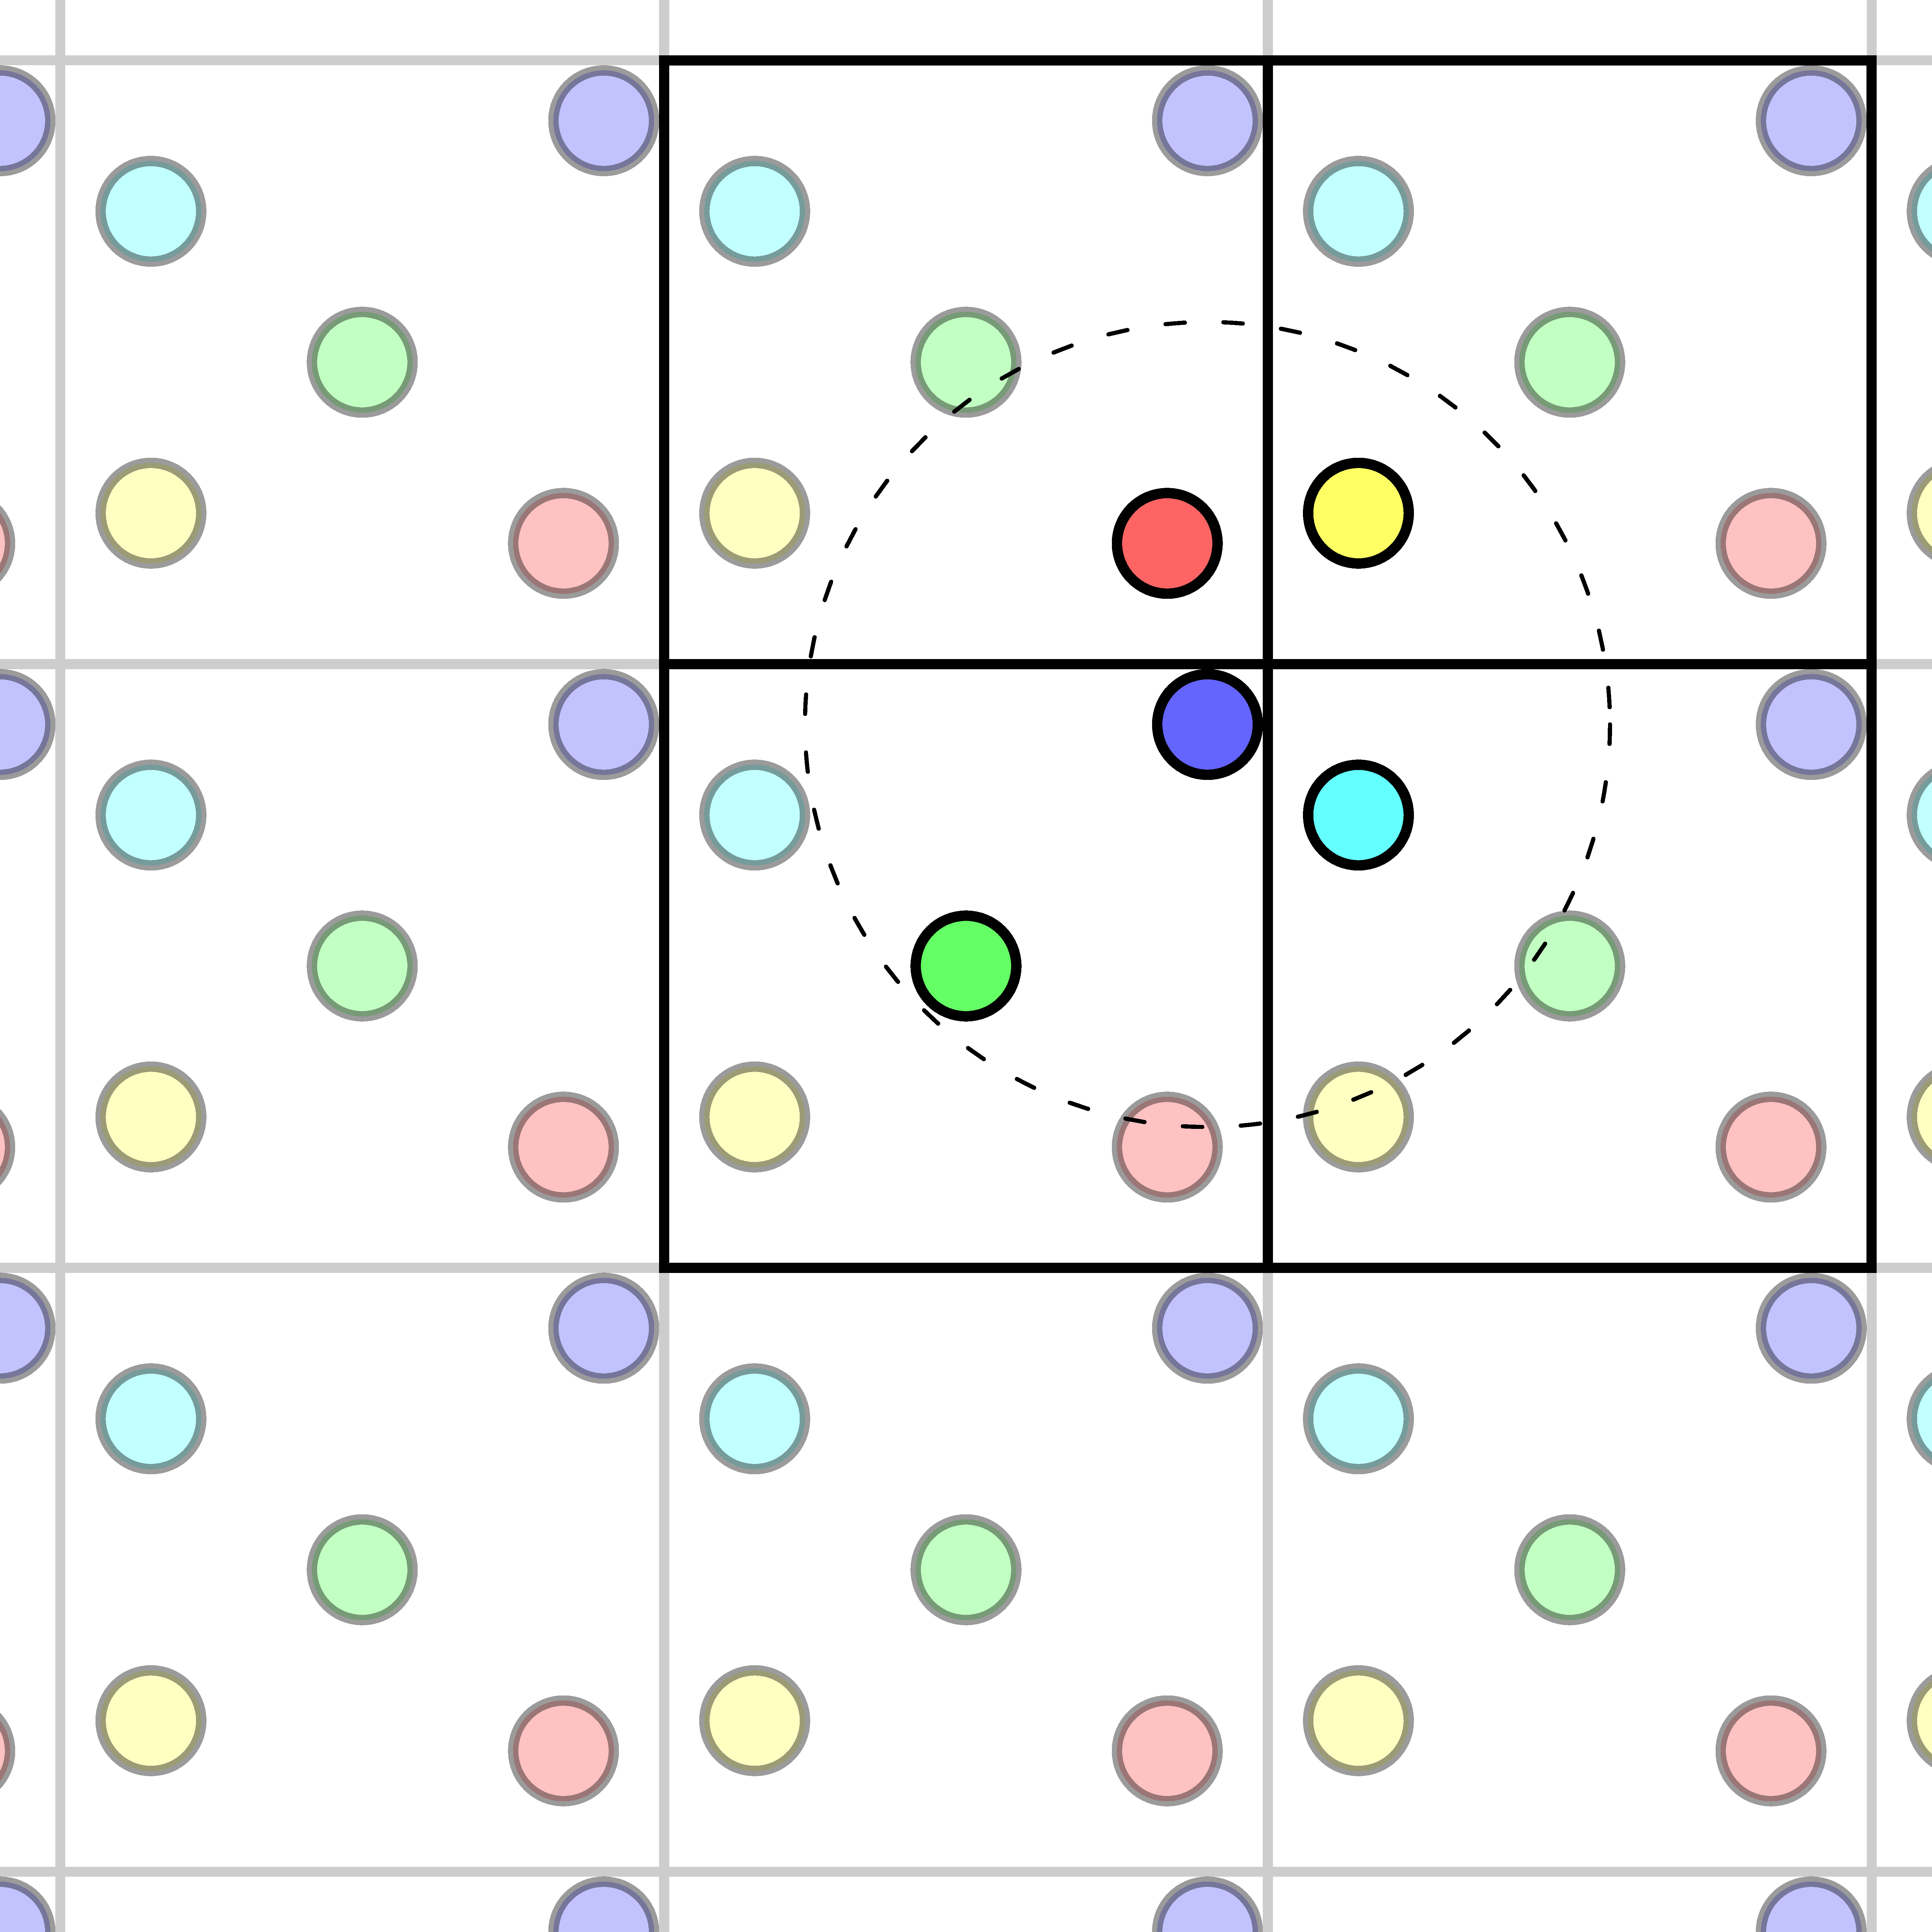
\includegraphics[width = 0.4\linewidth]{figures/pbc/pbc}
  \caption[Periodic boundary conditions schematic]{Schematic of a simulation using periodic boundary conditions.}
  \label{fig:periodic}
\end{figure}
At the scale of atomistic modelling, the materials being studied effectively stretch out infinitely relative to the scale of short-range and Coulombic interactions.
It is of course not feasible to model these systems as such, so boundary conditions which closely approximate this are needed.

Periodic boundary conditions (Figure \ref{fig:periodic}) take the contents of the simulation, and create copies of it at each boundary.
When calculating interactions, species in the ``main'' simulation are able to interact with other species in the main simulation, and those in the repeated simulations, subject to cutoff criteria applied to said interactions.
As the system is infinitely repeating, each copy of an atom must by definition be experiencing the same net force as each of its copies.
As such, it is sufficient to calculate the forces for a single cell only.

Another important of periodic boundary conditions is that atoms which would leave the boundaries of the simulation in the next iteration or time-step are reintroduced at the opposite boundary.
For Molecular Dynamics simulations (Section \ref{sec:MD}), this allows for atoms to move freely rather than being constrained to certain positions in order to keep a constant number of bodies in the simulation.
This is particularly useful when studying diffusion, allowing atoms near simulation boundaries to hop to all adjacent sites.


\newpage


\section{Point defects}
Whilst the atomistic modelling techniques already discussed are applicable in the generic case (as can be demonstrated by their suitability when applied to a P1 symmetry group), they have thus far only been discussed in the context of bulk systems.
In solid-state materials, it is often the presence of defects which gives rise to properties of interest, most likely in concentrations far too low to be studied in a periodic system.
As an example, the energy associated with the formation and migration of \ce{Li+} ions in candidate electrode materials is a key metric of their likely performance.

An overview of defect types, as well as the formalisms used in defining defect formation, is given in the appendix.

\subsection{Mott-Littleton method}
The Mott-Littleton method allows for the modelling of one or more defects at infinite dilution.
The perfect crystal structure is first solved using the techniques listed in Section \ref{sec:minimization}, and the converged result used as an initial condition.
Defects are then introduced the system is once more allowed to relax.
The difference in energy of the systems is directly attributable to the perturbation introduced, and is therefore the energy required to form the defect introduced.
Use of a small periodic system would repeat the defect and be equivalent to simulating the defect at high concentration.

Instead, the system is divided into three concentric spherical regions, as illustrated in Figure \ref{fig:mott}.
As the introduction of a single point defect removes symmetry from the system, a periodic approach is not appropriate, nor is the consideration of an infinite system.

\begin{figure}
  \centering
  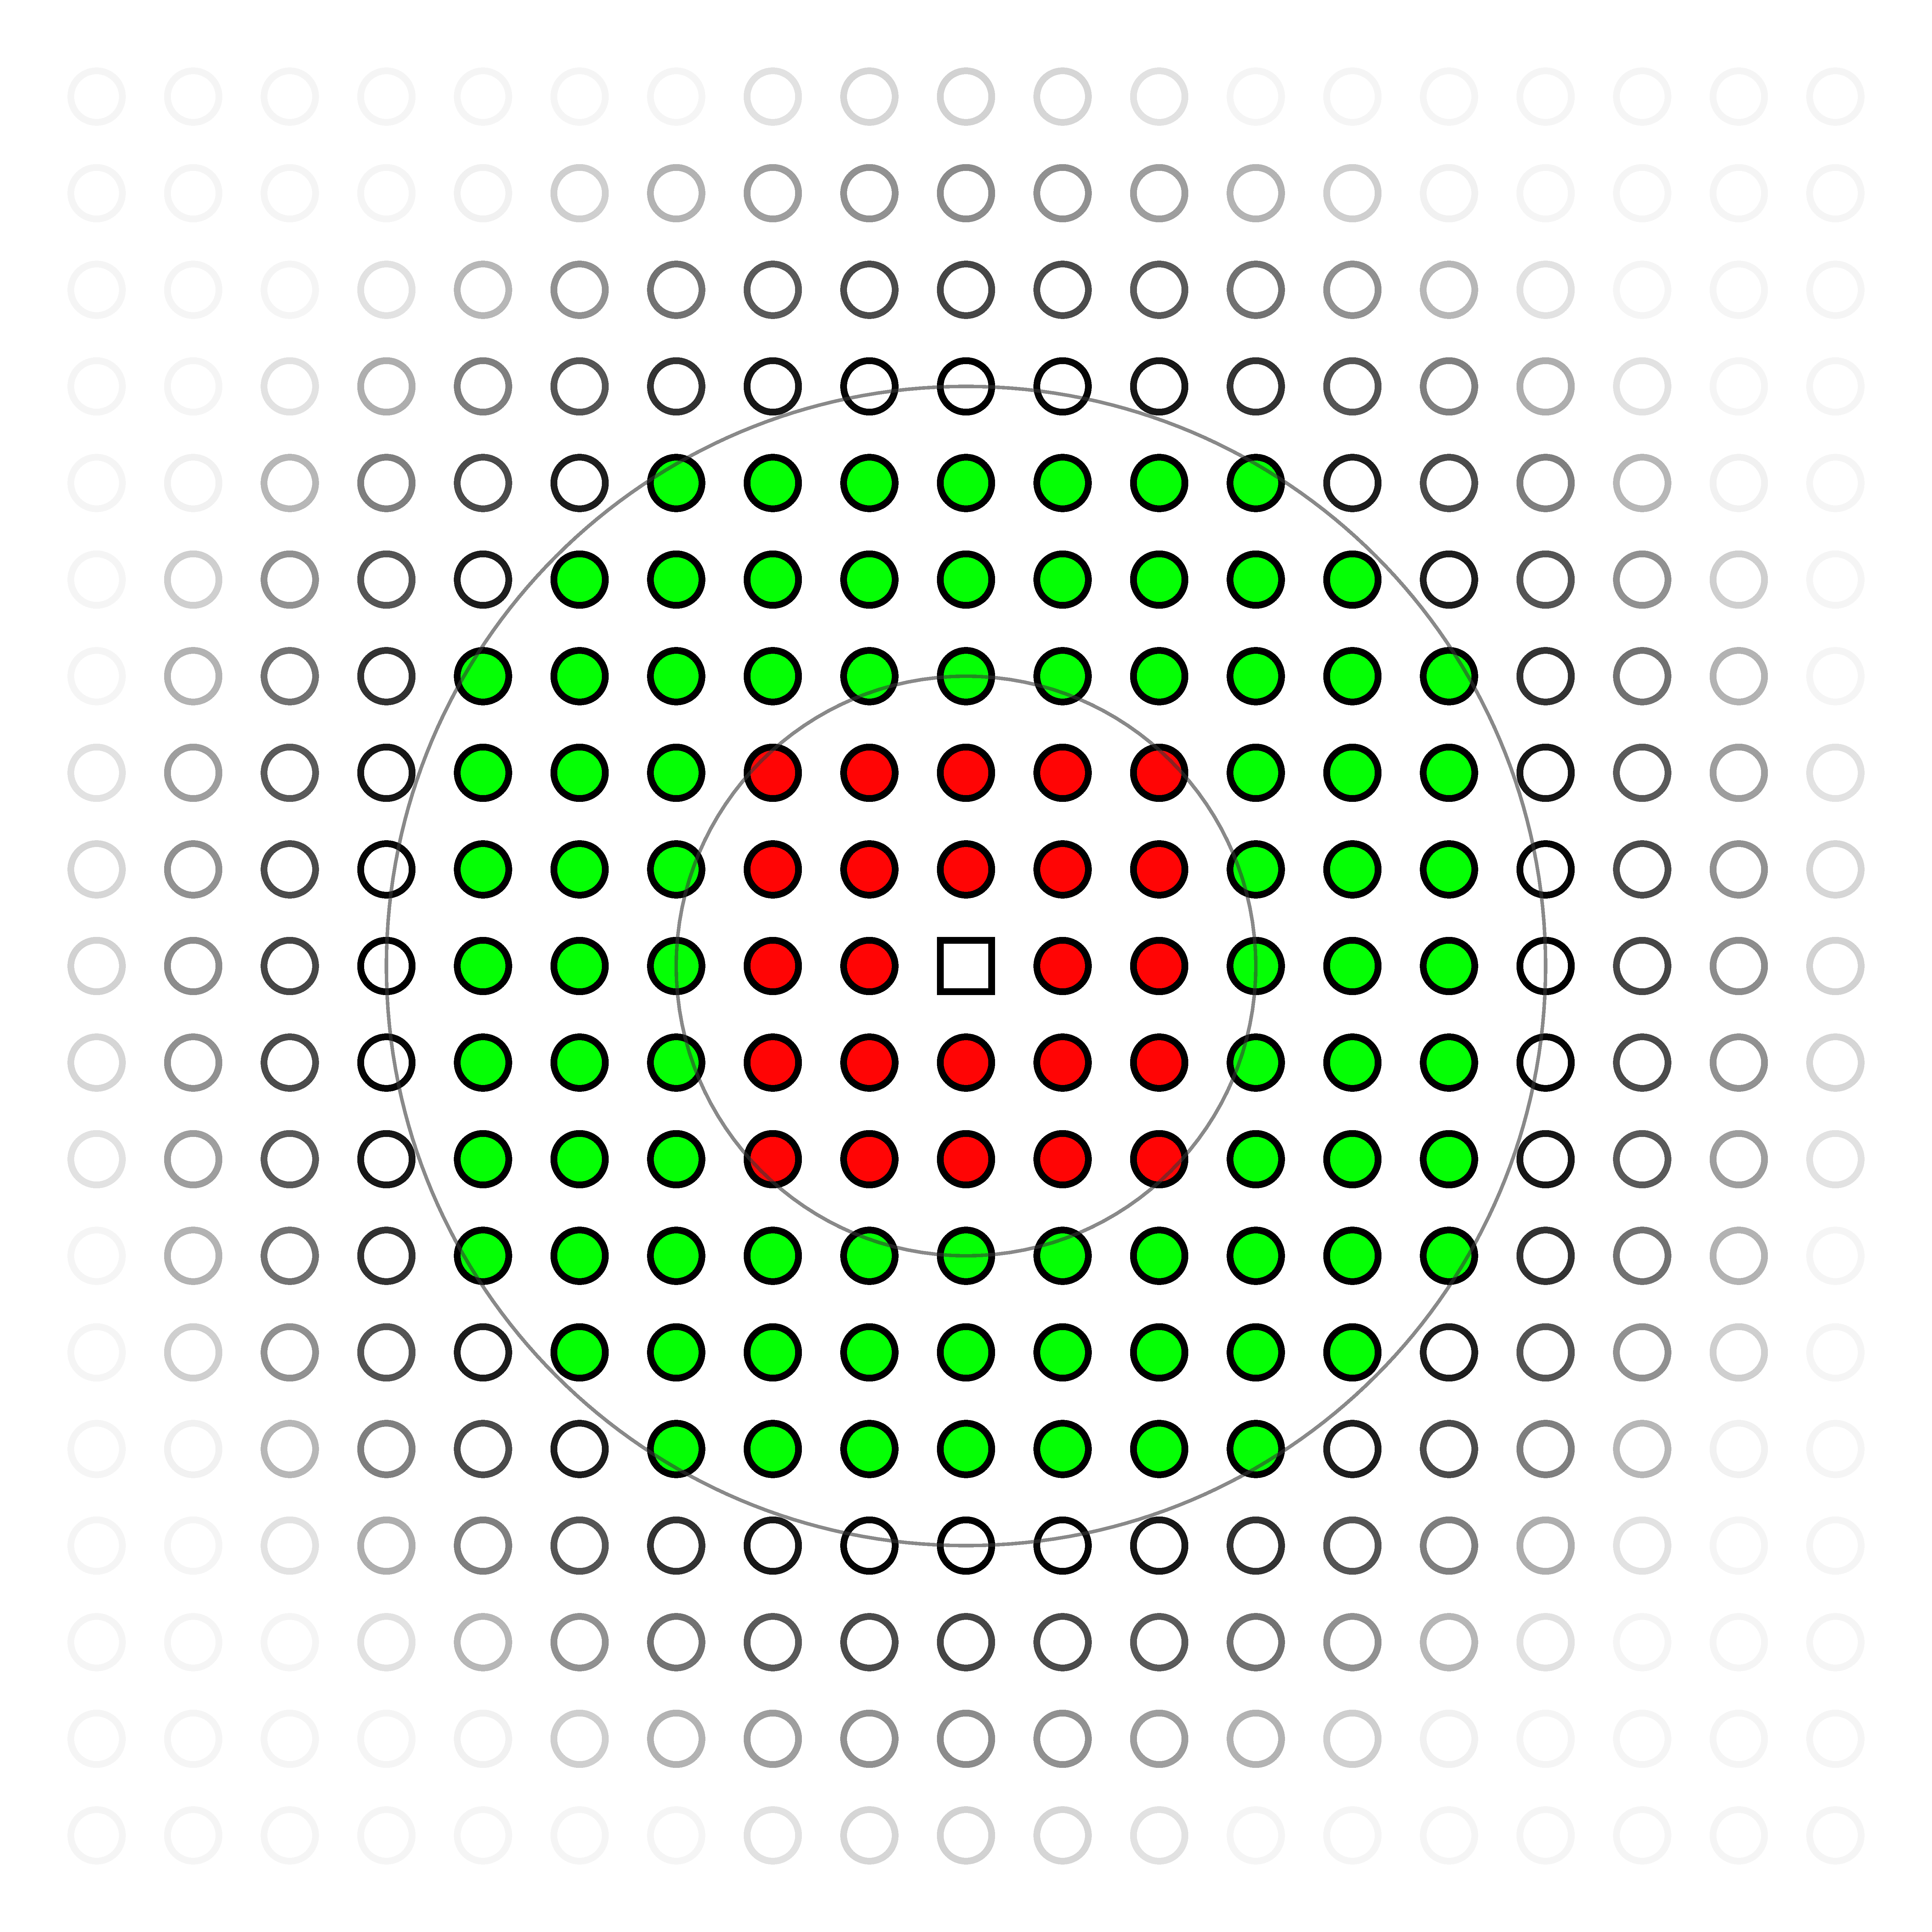
\includegraphics[width = \linewidth]{figures/mott/mott}
  \caption[Mott-Littleton method schematic]{Schematic illustrating the Mott-Littleton method. Ions in region I (green) are modelled explicitly using potential forms due to their proximity to the defect (square). Region IIb ions (white) are modelled using a continuum method. Region IIa ions (green) use a harmonic relationship, smoothing the transition from explicit (Region I) to implicit (Region IIb) modelling.}
  \label{fig:mott}
\end{figure}

Region I contains those ions closest to the defect.
Their close proximity to the defect means no simple approximation can be made to predict the defects impact.
As such, the relaxation of these species is modelled explicitly, using potential models and gradient descent techniques.

Ions in Region II are sufficiently far from the defect to be reasonably approximated using analytical methods.
Region IIb, the outermost region, is sufficiently far from the defect to only impacted by Coulombic interactions with the defect.
These are modelled using a dielectric continuum, the magnitude of the force experienced, and corresponding energy change, being a function of the net charge of the defect and the distance from the defect centre.


Ions in region IIa are modelled as having harmonic interactions with the defect, having an energy cost associated with their displacement from their initial position.
This region smooths the transition between the explicit modelling regime in region I and the implicit modelling regime in region IIb, avoiding discontinuities in the resultant energy surface.

The success of this technique relies upon selection of radii for the regions such that discontinuities do not occur between regions.
Selection of radii intervals greater than the cut-off values imposed on short range interatomic potentials typically achieves this.
That is to say, region IIa should be large enough such that no species in region I have any short range interactions with species in region IIb.

Further, the computational cost of relaxing region I is approximately of {\color{red}$O(r^2!)$}.
As such, a radius for region I should be chosen such that the resultant defect energy does not change with increasing radius, whilst being as small as possible to reduce simulation time.

\subsection{Supercell approach}  
Supercell methods simply take a large supercell of the repeating crystal unit and add a defect to this supercell.
The cell is then modelled as before, with the supercell repeating ``infinitely''.
This approach is limited in that in order to model low defect concentrations, a huge supercell is required.

As such, this method is generally instead only applied in Molecular Dynamics (Section \ref{sec:MD}), where a large concentration of Li vacancies are added in order to allow diffusion events to be observed.

\subsubsection{{\color{red}Symmetry optimisation}} %TODO rewrite
By their nature, crystal structures contain a number of symmetry elements.
In many cases, a number of interactions will be equivalent, enabling the number of computationally expensive operations to be reduced by simply treating some interactions as being equivalent and calculating them once rather than several times.
The addition of defects to a system reduces the overall symmetry of the structure, but there often still exist some symmetry elements.
Symmetry optimised algorithms are automatically implemented where appropriate in GULP.

\section{{\color{red}Molecular dynamics (MD)}}
\label{sec:MD}
Energy minimisation techniques are used to study systems at zero Kelvin.
As such, phenomenon arising only where ions have thermal energy cannot be studied with these techniques.

Molecular dynamics (MD) can overcome this issue by assigning each particle a velocity (usually subject to a Boltzmann distribution) and allows the system to evolve over time subject to some imposed constraints.
This in effect allows for phenomenon arising from thermal effects to be studied,
assigns and tracks kinetic energy of atoms, allowing the system to evolve over time.

The equation which fundamentally governs MD simulations is simply Newtons law of motion:
\begin{equation}
	\mathbf{F} = m\mathbf{a}
\end{equation}

As the force each particle is a function of the positions of each particle in space, which in turn evolves as a function of time, it is necessary to solve this equation repeatedly.

The force acting on each particle is assumed to be constant for some small period of time $\Delta t$.
With this assumption, the position and velocity of each particle at time $t+\Delta t$ can using an Euler integration scheme by:
\newpage
\subsection{Integration schemes}
The Taylor expansion is a technique which allows a function to be expressed as a infinite sum of terms calculated from that functions derivatives at a given point:
\begin{equation}
f(t) = f(t_0 + \Delta t) = \sum_{n=0}^\infty \frac{1}{n!}f^{(n)}(t_0)\Delta t^n
\end{equation}
Applying this to the position of atoms in the system as a function of time yields:
\begin{align}
\mathbf{x}(t_0 + \Delta t) &= &x(t_0) \; &+ &x'(t_0)\Delta t \;&+& &\frac{1}{2}x''(t_0)\Delta t^2 \;&+& \frac{1}{6}x'''(t_0)\Delta t^3& +\;\dots\\
                           &= &x_{t_0} \; &+  &v_{t_0}\Delta t \;&+&   &\frac{1}{2}a_{t_0}\Delta t^2     \;&+& \frac{1}{6}j_{t_0}\Delta t^3& +\;\dots
\end{align}
Truncating this expansion at different terms yields a series of potential equations which can be solved, the discarded terms constituting the error in each step.
The lowest order discarded term will determine the magnitude of the error, with ``simpler'' expansions requiring a correspondingly smaller $\Delta t$ in order to reduce the magnitude of the error to an acceptable value.

\paragraph{Euler integration}
Truncating the Taylor expansion of the position and velocity of particles as a function of time at the first term gives an Euler integration scheme:
\begin{equation}
	\mathbf{v}_{t +\Delta t} = \mathbf{v}_t + \frac{d\mathbf{v}}{dt}\Delta t = \mathbf{v}_t + \mathbf{a}_t\Delta t +\Theta(\Delta t^2)
	\end{equation}
\begin{equation}
	\mathbf{x}_{t +\Delta t} = \mathbf{x}_t + \frac{d\mathbf{x}}{dt}\Delta t = \mathbf{x}_t + \mathbf{v}_t\Delta t +\Theta(\Delta t^2)
\end{equation}
With $\Theta$ representing the error, the brackets indicating the relationship between the size of the error and the choice of time step.
Unfortunately, the $\Theta(\Delta t^2)$ error terms in this integration scheme require a prohibitively small $\Delta t$ to be used for all but the simplest of systems. 

\paragraph{Verlet algorithm} A commonly used integration scheme, the Verlet algorithm, instead truncates the Taylor expansion of the atom positions at the third derivative:
\begin{equation}
\mathbf{x}_{t + \Delta t} = x_{t} \; +  v_{t}\Delta t \;+ \frac{1}{2}a_{t}\Delta t^2     \;+ \frac{1}{6}j_{t}\Delta t^3 + \Theta(\Delta t^4)
\label{eq:verlet1}
\end{equation}
with $j$ indicating the ``jerk'', or rate of change of acceleration of the function.
As the rate of change of acceleration is related to the rate of change of force, the jerk term is not readily calculated.
The Verlet algorithm overcomes this issue by using information known about the system in previous time steps $t_{t}$:
\begin{equation}
\mathbf{x}_{t - \Delta t} = x_{t} \; -  v_{t}\Delta t \;+ \frac{1}{2}a_{t}\Delta t^2     \;- \frac{1}{6}j_{t}\Delta t^3 + \Theta(\Delta t^4)
\label{eq:verlet2}
\end{equation}

Summing equations \ref{eq:verlet1} and \ref{eq:verlet2} yields:
\begin{align}
\mathbf{x}_{t + \Delta t} + \mathbf{x}_{t - \Delta t} &= 2x_{t} + a_{t}\Delta t^2 + \Theta(\Delta t^4)\\
\mathbf{x}_{t + \Delta t} &= 2x_{t} + a_{t}\Delta t^2 -  \mathbf{x}_{t - \Delta t} + \Theta(\Delta t^4)
\label{eq:verlet}
\end{align}

\noindent allowing for the positions of particles to be calculated at the next time step.
Interestingly, this integration scheme not only obviates determining the rate of change of acceleration of particles, it also skips the calculation of the velocity term.
The Verlet integrator is also time reversible and symplectic (preserves energy), making it suitable for the dynamic systems encountered in MD.
Of course, in order to calculate the kinetic energy of the system, knowledge of particle velocities is needed.
Subtraction of equation \ref{eq:verlet2} from \ref{eq:verlet2} yields:
\begin{equation}
	v_{t} = \frac{x_{t+\Delta t} - x_{t-\Delta t}}{2\Delta t} + \Theta(\Delta t^2)
\end{equation}
giving the Verlet velocity.
As with the $\Theta(\Delta t^2)$ term being too large for calculating the position with a Euler integration scheme, the error term here requires prohibitively small time steps for complex systems.
Velocities are to determine the temperature of the system, which in turn must be a conserved quantity in certain ensembles. %TODO

\paragraph{Velocity Verlet} The Velocity-Verlet algorithm explicitly calculates velocities at half time steps:
\begin{align}
	v_{t +\frac{1}{2}\Delta t} &= \frac{x_{t+\Delta t} - x_t}{\Delta t}\\[10pt]
	&= v_t + \frac{1}{2}a_t\Delta t + \Theta(\Delta t^3)
\end{align}
This half-velocity, the predicted velocity at the time half way between the current and next time step, is then used to update the current positions of ions in the system as in a Euler scheme:
\begin{equation}
	x_{t+\Delta t} = x_t + v_{t +\frac{1}{2}\Delta t}\Delta t + \Theta(\Delta t^4)
\end{equation}

\noindent The velocity at the next time step is then calculated by:
\begin{equation}
	v_{t + \Delta t} = v_{t +\frac{1}{2}\Delta t} + \frac{1}{2}a_{t+\Delta t}\Delta t + \Theta(\Delta t^3)
\end{equation}

\noindent Explicitly calculating the velocities in this manner maintains the order of the error in the particle positions, whilst increasing the order of the error in the velocity terms.

\subsection{Timestepping and equilibriation}
The choice of time step will strongly influence the output of an MD simulation. 
Selection of an excessively small $\Delta t$ will result in simulations being too expensive to observe phenomenon which occur over large time periods such as bulk diffusion.
Counter to this, too large a $\Delta t$ can allow for atoms to occupy unphysical states.
For example, as the Velocity Verlet algorithm only evaluates forces at $x_{t}$ and $x_{t +\Delta t}$,  a particle with low kinetic energy may skip over an large energy barrier present at $x_{t +\frac{1}{2}\Delta t}$ if allowed to move too great a distance between time steps.
Typically, selecting time steps an order of magnitude below the period of atomic vibrations (\SIrange{0.1}{1}{\femto\second}) prevents unphysical phenomenon at the least computational expense.

\subsection{Initialisation and equilibration}
Prior to useful information being obtained fron an MD simulation, the system must be initialised and allowed to equilibrate.
This is generally done in a number of steps:
\paragraph{Structure generation}
Phenomenon of interest in battery materials, such as Li ion diffusion, occur over large length scales and are studied using statistical techniques.
As such a supercell approach is generally used to provide the sufficient bodies and space for these phenomenon to be observed.
Relaxed structures from energy minimisation codes, using the same potential forms as are used in the MD simulation, are commonly used as the repeating unit here.
In disordered solids, this step is non-trivial, with the configuration space of a typical MD simulation far exceeding that explorable by \textit{ab initio} methods.
Techniques allowing for low energy local structures to be characterised and ``tiled'' may be a technique to allow pseudo-random structure generation; an interesting avenue for future work, but not implemented as of yet.

\paragraph{Introduction of defects}
For diffusion to be observed, a key phenomenon in battery materials, some mobile species vacancies must be introduced.
Mobile species can then hop to these vacant sites, allowing ionic motion to be characterised.
The location of these defects is randomly assigned in this study, where bulk phenomenon are of interest.
The introduction of these defects must be charge compensated.
As MD does not explicitly calculate electron densities, it is not possible to associate the charge compensation with a specific set of atoms.
Instead the charge is ``smeared'' across all species which could have changed oxidation state for a given vacancy concentration.
As an example, in the case of introducing 10\% Li vacancies to a \ce{LiCoO2} cathode, a charge of $+0.1$ per formula unit must be assigned to the Co ions, giving an overall oxidation state of \ce{Co^{3.1}+}.

A second energy minimisation must then be performed to allow the structure to relax locally around the vacancies introduced.

\paragraph{Initialisation}
None of the integration schemes discussed are ``self-starting'', that is to say, they are reliant on some initial velocities being known in order to be used.
For a system containing $N$ bodies, velocities will be randomly assigned to give the system a desired initial temperature subject to:
\begin{equation}
	\sum^N_{i=1}m_i\mathbf{v}_i^2 = 3Nk_bT
	\label{eq:boltz}
\end{equation}
whilst ensuring the system has no net momentum in any vector:
\begin{equation}
	\sum^N_{i=1}m_i\mathbf{v} = 0
\end{equation}

While these velocities ensure that the desired kinetic energy is present in the initial steps of the simulation, it does nothing to prevent the assignment of unphysical velocities.
In order to prevent this biasing the results obtained, the simulation is allowed to run until a pseudo-steady state is reached. 
The number of steps necessary to obtain this is strongly case dependent, but can usually be visually identified in the data and discarded manually if necessary.

\subsection{Ensembles}
An ensemble is the set of all accessible states a simulation might access given sufficient time, subject to some constraints.
Selection of appropriate constraints enables a series of simulations to probe a system of interest across a range of specified conditions.
\paragraph{Canonical (NVT) ensemble}
The canonical ensemble keeps constant the number of bodies (N), the volume (V) of the simulation cell, and the temperature of the simulation (calculated by Equation \ref{eq:boltz}).
Whilst the number of bodies and cell volume are readily preserved, the internal energy and thus temperature may change over time due to rounding errors in the integration method.

\paragraph{Isobaric-isothermal (NPT) ensemble}
The Isobaric-isothermal ensemble keeps constant the number of bodies (N), the pressure (P) of the simulation cell, and the temperature of the simulation (calculated by Equation \ref{eq:boltz}).
In this instance, both the pressure and temperature of the system need adjusting over time.

A naiv{\"e} approach to maintain temperature is to calculate the temperature at each time step, and scale the velocities of each particle accordingly.
This technique prevents any temporary deviations in temperature, which is an unrealistic constraints.

A more realistic approach is to use a thermostat, coupling the system to a heat sink at the target temperature.
The rate of change of instantaneous velocity is then given by:
\begin{equation}
\frac{dT_{t}}{dt} = \frac{1}{\tau}(T_{sink} - T_t)
\end{equation}
where $\tau$ is in effect a gain term for a proportional controller attached to the system.
Similarly, the system pressure can be controlled by scaling the atomic coordinates of each particle subject to:
\begin{equation}
\frac{dP_{t}}{dt} = \frac{1}{\tau}(P_{sink} - P_t)
\end{equation}
\newpage
\subsection{Analysis}
In order to extract useful information from MD simulations, analysis of the positions of atoms as a function of time must be undertaken.
A number of key parameters are calculated, from which interesting material properties can be derived.
\paragraph{Mean square displacement}
The mean square displacement (MSD) measures the distance each atom has moved from its position at a given time, usually treating $t_0$ as the first time step after the equilibration period.
The MSD for an $N$ body system at time $t$ is defined as:
\begin{equation}
	MSD_t = \langle (\mathbf{x}_t - \mathbf{x}_0)^2 \rangle = \frac{1}{N}\sum_{i=1}^N(x_{i, t = t} - x_{i, t = 0})^2
\end{equation}
The MSD can be calculated for the system as a whole, or for a specific subset of particles.
By calculating the diffusion coefficient associated with all the particles of a given species, the self-diffusion coefficient of that species, for d-dimensional diffusion, is then given by:
\begin{align}
	MSD_t &= 2dDt\\[5pt]
	D &= \frac{MSD_{t_2} - MSD_{t_1}}{2d(t_2 - t_1)}t
\end{align}

The activation barrier associated with an average site hopping event can then be found by plotting the natural logarithm of the diffusion coefficient versus the inverse temperature:
\begin{equation}
	\ln{D} = \frac{-E_a}{R}\cdot\frac{1}{T} + \ln{A}
\end{equation}

This activation energy may offer insights into migration barriers not accessible in zero Kelvin calculations.
\paragraph{Time averaged densities}
Given the vast quantities of data obtained over a moderate length MD simulation, visualisation techniques which allow for features persistent across the entire simulation are particularly useful.
One such technique, time averaged density plots, discretises the simulation domain and calculates the probability that a given species will be found in each subdomain at any given time.
Visualising this data thresholding to include only those regions with a high probability of containing species of interest, allows for migration pathways between lattice sites to be identified.
\section{Potential fitting}
In order for simulations to provide valuable insights into the material being studies, the potential forms used closely approximate the true energy surface.
Whilst some universal forcefields are available, the phenomenon of interest in cathode materials cannot be adequately replicated with these.
As such, unless some potentials developed for the same or similar systems is already available, some new potentials must be derived for the system or class of systems being studied.

\subsection{Basis}
In order to fit a potential, some prior information about the system must be available. 
If experimental data is available for material of interest, it is possible to fit potentials to this.
Crystallographic data provides atomic coordinates and unit cell parameters which, if replicated by a given set of potential, serve as a good metric of performance.
Of course, the number of degrees of freedom associated with a typical potential set is large, so crystallographic data may not be sufficient to yield a unique potential set.
Dielectric constants, elastic constants and other easily measured parameters may also serve as a basis for fitting.

In the absence of experimental data, such as in screening studies, \textit{ab initio} studies can be used as a substitute. 
In this case, it is possible to fit directly to the potential energy surface the \textit{ab initio} yields.

\subsection{Selection of potential form}
The selection of potential forms will influence the quality of fit, with more complex potential forms able to more closely replicate the energy surface of the basis information.


\subsection{Metrics}
In order to distinguish between sets of potential parameters, an appropriate metric must be selected.
Some commonly used metrics to compare the basis information and calculated structure:
\begin{labeling}{\textbf{Atomic displacements}}
	\item [\textbf{Lattice parameters}] The length and angles of the unit cell basis vectors
	\item [\textbf{Atomic displacements}] Cartesian or fractional displacement of each atom
	\item [\textbf{Forces}] The magnitude and direction of the force on each atom
\end{labeling}
Some or all of these metrics can be used, depending on the quality and nature of the basis information.
For example, while forces can be used as a metric for fitting using crystallographic data as a basis, all forces will be zero in this case, so use of \textit{ab initio} data may be preferable for this metric, allowing the potential to be fit to a wider range of interatomic separations.

A generic cost function can then be defined as:
\begin{equation}
	F = \sum_{n=1}^{N_{obs}}w_i(f_i^{obs} - f_i^{calc})^{n_i}
\end{equation}

Where $w_i$ is a weighting term, increasing the bias of the fit towards matching certain observables.
$n_i$ can be set as 1 to give a linear fit, where the cost function is simply the sum of the error of the observables, or 2, giving the sum square of errors which more heavily penalises large errors in a given observation.

\subsection{Search algorithms}
A number of pre-existing strategies for searching the parameter space (analogous to the configuration space discussed in Section \ref{sec:minimization}).
Many of the techniques discussed in that section can also be applied to this problem.
Of course, unlike in energy minimisation simulations where a reasonable initial condition can be determined, it is often the case in potential fitting that minimal prior information is available, or it is not possible to arrive at some initial conditions intuitively.
In such cases, local optimisers, which are reliant on the path of steepest descent leading to the global minima if the global minima is to be obtained, may not be appropriate.
Global optimisers, such as genetic algorithms and Monte-Carlo techniques may be appropriate in these conditions.
Pairing global optimisers (to broadly sample the parameter space), with local optimisers (to improve on the quality of parameters yielded by the global optimiser) is one way of overcoming the limits of local optimisers while limiting the cost of global optimisers.

A limitation of all these approaches is that unless the selected potential form is such that all the basis data can be perfectly and uniquely replicated by a given parameter set, it is expected that the cost function surface will contain numerous local minima.
This is especially likely where experimental data is being used, introducing some degree of random error to the basis information.

An approach currently in development by the author, in collaboration with Dr. Benjamin Morgan and Dr. Lucy Morgan, is to use Bayesian techniques to derive interatomic potentials.
Sequential Monte Carlo for Approximate Bayesian Computation (SMC-ABC),\cite{Toni2009a} in contrast to frequentist approaches, preserves the uncertainty inherent in deriving an interatomic potential.

Instead of yielding a single parameter set by gradient descent or similar, in SMC-ABC each parameter is modelled as being described by some initially broad statistical distribution.
Parameter sets are sampled from these prior distributions, and those which adequately replicate the basis data sets are used to update the prior distribution, biasing the new distribution to more frequently give parameter values close those used in accepted trials.
Iteratively applying this procedure yields distributions for each parameter being fitted, which correspond not to values which are necessarily the global minimum, but those values which offer good agreement with the basis data with low sensitivity to the values of the other fitted parameters.
This is therefore suitable for fitting to data with some inherent error, and for cases where overfitting leads to the selection of potential parameters which are not robust to new data.



\bibliographystyle{rsc}

\bibliography{library}
\pagestyle{empty}
\end{document}